\documentclass[%
	corpo=12pt,
    twoside,
    stile=classica,
    oldstyle,
    tipotesi=custom,
    greek,
    evenboxes,
]{toptesi}
%%%%%%%%%%%%%%%%%%%%%%%%%%%%%%%%%%%%%%%%%%%%%%%%%%%%

\usepackage[utf8]{inputenc}
\usepackage[T1]{fontenc}
\usepackage{lmodern}
\usepackage{float}
\usepackage{hyperref}

\usepackage{hyperref}
\hypersetup{%
    pdfpagemode={UseOutlines},
    bookmarksopen,
    pdfstartview={FitH},
    colorlinks,
    linkcolor={blue},
    citecolor={blue},
    urlcolor={blue}
  }

%%%%%%% use PDFLATEX 

\usepackage{lipsum} %to insert random text
\usepackage[section]{placeins}

\usepackage{geometry} %for the margins
\newcommand\fillin[1][4cm]{\makebox[#1]{\dotfill}} %for the dotted line in the frontispiace

\usepackage{dcolumn}
\newcolumntype{d}{D{.}{.}{-1} } %to vetical align numbers in tables, along the decimal dot

\usepackage{amsmath}

\usepackage{natbib} % for the bibliography
\bibliographystyle{plainnat}


%%%%%%% Local definitions
\newtheorem{osservazione}{Osservazione}% Standard LaTeX
\newtheorem{observation}{Observation}% Standard LaTeX




%%%%%%%%%%%%%%%%%%%%%%%%%%%%%%%%%%%%%%%%%%%%%%%%
%%%%%%%%%%%%%%%%%%%%%%%%%%%%%%%%%%%%%%%%%%%%%%%%



\begin{document}\errorcontextlines=9
%\english

\begin{titlepage}
\newgeometry{left=1cm,right=1cm,top=3cm,bottom=3.5cm}  %specific margins for this page

\begin{center}

{\huge POLITECNICO DI TORINO}\\[1.5cm]
\textbf{Corso di Laurea\\in Ingegneria Matematica}\\[3cm]
%\textbf{Corso di Laurea Magistrale\\in Ingegneria Matematica}\\[3cm]

{\Large Tesi di Laurea}\\[1cm]
%{\Large Tesi di Laurea Magistrale}\\[0.5cm]
\textbf{\LARGE Modelli predittivi della saliency nelle rappresentazioni grafiche dei dati }\\[2cm]
\includegraphics[width=0.2\textwidth]{./Pictures/logo_polito.jpg}
\vspace{3cm}


\begin{minipage}{0.85\textwidth}
\begin{flushleft}\large
\textbf{Relatori} \hfill \textbf{Candidato}\\
prof. Fulvio Corno \hfill  Samuel Grassi \\
prof. Luigi De Russis \\
prof. Luisa Fernanda Barrera Leon \\
\textit{firma dei relatori} \hfill \textit{firma del candidato}\\[0.35cm]
\fillin\ \hfill \\
\fillin\ \hfill \\
\fillin\ \hfill \fillin
\end{flushleft}
\end{minipage}

\vfill

Anno Accademico 2020-2021
\end{center}

\restoregeometry %restor default margins 

\end{titlepage} %the frontispiece

%%%%%%% Dedication
\ifclassica%
{\begin{dedica}
     
\end{dedica}
%%%%%%% 

%\renewcommand{\sommario {SSOM}}%summary
%\sommario
\abstracttile{\Huge{\textbf{Obiettivo}}}
\\\\
\\\\
%Here goes the abstrat of your thesis
L'obiettivo di questo lavoro di Tesi è quello di approfondire ed entrare nel dettaglio dell'argomento della \textit{saliency}, in particolare della \textit{pre-attentive saliency}, riguardo all'analisi e la distribuzione dei punti di fissazione di un osservatore su grafici di business.

Inizialmente il focus era quello di cercare di trovare un algoritmo competitivo con alcuni modelli sulla saliency visiva già proposti (Itti, Matzen), ma in seguito, dopo aver analizzato i risultati su un dataset già esistente (\textit{MASSVIS}), ci si è concentrati sul valutare attentamente le performance di questi modelli già esistenti su un nuovo esperimento creato e controllato da noi. 

Infine, alla luce di quanto trovato e del materiale prodotto, il lavoro si conclude con alcuni spunti e proposte contenenti alcuni punti sui quali ci si potrebbe andare a focalizzare per produrre una modifica che effettivamente sia confrontabile o addirittura migliore di ciò che è già disponibile. 

%%%%%%%%%%%%%%%%%%%%%%%%%%%%%%%%%%%%%%%%%%%%%%%%
%%%%%%%%%%%%%%%%%%%%%%%%%%%%%%%%%%%%%%%%%%%%%%%%

%\ringraziamenti%acknowledgements
%%Acknowledge the people you love and/or work with
%I candidati ringraziano vivamente il Granduca di Toscana per i mezzi messi loro a disposizione, ed il signor Von Braun, assistente del prof.~Albert Einstein, per le informazioni riservate che egli ha gentilmente fornito loro, e per le utili discussioni che hanno permesso ai candidati di evitare di riscoprire l'acqua calda.

%%%%%%%%%%%%%%%%%%%%%%%%%%%%%%%%%%%%%%%%%%%%%%%%
%%%%%%%%%%%%%%%%%%%%%%%%%%%%%%%%%%%%%%%%%%%%%%%%

\tablespagetrue\figurespagetrue%to include the list of tables
%and the list of figures - yuo can comment these commands

\indici%table of content
%It automatically generated

%%%%%%%%%%%%%%%%%%%%%%%%%%%%%%%%%%%%%%%%%%%%%%%%
%%%%%%%%%%%%%%%%%%%%%%%%%%%%%%%%%%%%%%%%%%%%%%%%

%Citation
%If you feel like a poetic guy!
%\ifclassica   
%\begin{citazioni}
%    \textit{If you cannot understand my\\argument, and declare}\\
%    it's Greek to me\\
%    \textit{you are quoting Shakespeare.}
%    
%    [\textsc{B. Levin}, Quoting Shakespeare]\vspace{1em}
%\end{citazioni}
%\fi

%%%%%%%%%%%%%%%%%%%%%%%%%%%%%%%%%%%%%%%%%%%%%%%%
%%%%%%%%%%%%%%%%%%%%%%%%%%%%%%%%%%%%%%%%%%%%%%%%

\mainmatter

%\part{Prima Parte}

\chapter{Concetti fondamentali}

%\section{Saliency}
Un obiettivo fondamentale della visualizzazione e di chi pubblica grafici di dati è quello di produrre immagini che contengano dati che favoriscano l'analisi visiva, l'esplorazione e la scoperta di nuove informazioni. In questo contesto, un ruolo importante è sicuramente ricoperto dalla percezione visiva umana. Come la persona vede e percepisce i dettagli in un'immagine può direttamente impattare sull'efficacia dell'osservazione. Una conoscenza della percezione visiva può migliorare significativamente la qualità e la quantità delle informazioni che vengono mostrate sull'immagine. Quello che noi esseri umani vediamo con i nostri occhi è fortemente influenzato dalla direzione in cui stiamo guardando e dove la nostra attenzione è focalizzata. Un altro aspetto di cui tenere conto è anche ad esempio che cosa ci aspettiamo di trovare in un'immagine prima ancora di andare ad osservarla.

Dopo numerosi studi e anni di ricerca si è notato che in ogni momento la visione dettagliata per forme e colori è possibile solo in una piccola porzione del campo visivo che i nostri occhi sono in grado di osservare. In pratica per riconoscere queste due caratteristiche, l'occhio umano scansiona piccole porzioni alla volta dell'immagine che si sta fissando. 

Un'importante scoperta è stata quella di identificare un insieme di caratteristiche visive che sono individuate rapidamente in una prima osservazione di basso livello. Queste sono state inizialmente chiamate \textit{preattentive} dato che la loro identificazione avviene prima ancora che l'attenzione si concentri sull'immagine. Tipicamente si considera \textit{preattentive}  tutto ciò che si verifica nei primi 200-250 ms. Alcune proprietà degli oggetti presenti in un'immagine che sono classificate \textit{preattentive} sono ad esempio: l'orientazione, la lunghezza, la dimensione, il colore, le ombre e alcune altre caratteristiche degli oggetti elencate nel documento [1]. Interessante sottolineare come se queste caratteristiche vengano combinate nella stessa immagine, potrebbero non più essere identificabili in maniera rapida rispetto a quanto avviene quando si presentano da sole. Queste proprietà sono state usate in esperimenti per i seguenti scopi: 
\begin{itemize}
\item \textit{target detection}, in cui gli osservatori sono chiamati a ricercare un elemento con un'unica caratteristica visiva;
\item \textit{boundary detection},  in cui gli osservatori devono dividere in due gruppi gli oggetti che presentano almeno una caratteristica in comune tra i due gruppi;
\item \textit{region tracking}, dove lo scopo è quello di tenere traccia di un oggetto che si muove nello spazio e nel tempo; 
\item \textit{counting and estimation}, dove l'obiettivo è riuscire a contare il numero di elementi di un'unica caratteristica visiva.
\end{itemize}

Ci sono varie teorie che cercano di spiegare come il processo \textit{preattentive} influenzi il sistema visivo.

Treisman ha proposto un modello dell'attenzione umana nel basso livello dell'osservazione. Questo è composto da un insieme di \textit{feature maps} (ognuna legata ad una precisa caratteristica visiva e possono agire in parallelo) e una \textit{master map of locations} (che invece introduce il concetto di posizione sull'immagine). Ha in più affermato che l'ammontare della differenza tra il target e i distrattori presenti sull'immagine influisce sul tempo di ricerca (come è normale che uno si aspetti).

Julész ha teorizzato come la prima parte della visione vada ad individuare tre categorie di proprietà visive chiamate \textit{textons}: le intersezioni tra le linee; i terminatori delle linee; le forme (linee, rettangoli, ellissi \dots) con specifica tonalità, orientazione e così via. In particolare ha aggiunto che a suo parere solo una differenza tra vari \textit{textons} possa essere notata nella fase \textit{preattentive}. 

Duncan e Humphreys hanno invece asserito che il tempo di ricerca di un target è basato su due criteri: la similarità T-N e la similarità N-N. La prima è la somiglianza tra gli obiettivi (\textit{targets}) e i non obiettivi (\textit{nontargets}). La seconda è la similarità che è presente solo tra i \textit{nontargets}. La variazione di una delle due influisce anche un pò sull'altra, però in generale quando la similarità T-N aumenta allora il tempo di ricerca diminuisce e la stessa cosa succede quando quella N-N decresce. In più, i due ricercatori hanno proposto una teoria sulla selezione visiva organizzata in tre step: il campo visivo è segmentato in parallelo; l'accesso alla memoria visiva a breve termine è una risorsa limitata; una scarsa corrispondenza tra una zona e uno schema di ricerca di alcune proprietà visive porta ad automatiche esclusioni di zone che sono legate con quella esclusa.

Più recentemente Wolfe ha invece designato l'idea della ricerca guidata ed è la prima volta in cui gli obiettivi dell'osservatore sono stati inseriti in un modello sulla ricerca visiva umana. Ha ipotizzato che una \textit{activation map} basata sull'approccio \textit{bottom-up} (ciò che emerge automaticamente dall'immagine) e su quello \textit{top-down} (quello che è legato alla consapevolezza di chi guarda) si costruisse durante la visualizzazione, con dei picchi di intensità dove l'attenzione ricade maggiormente. Come Triesman, anche Wolfe crede che l'immagine venga divisa in \textit{feature maps} che poi ricombinate insieme generano i picchi sulla \textit{activation map}.

Huang ha poi presentato un nuovo modello di visione a basso livello concentrandosi sul cercare di capire per quale motivo spesso sull'immagine ci si concentra su delle cose che in realtà non sono rilevanti con quello che in realtà interessa. La teoria divide la ricerca visiva in due parti: selezione e accesso. Durante la prima fase si selezionano un insieme di oggetti dalla figura, mentre nella seconda si determina quale proprietà degli oggetti selezionati un osservatore può apprendere. Huang ha poi continuato affermando che il sistema visivo può suddividere l'immagine tra gli oggetti selezionati e quelli esclusi, per poi accedere a certe proprietà solo per i selezionati. Questa è la base che sta dietro alla \textit{boolean map}.

Un aspetto rilevante che sta alla base della visione di basso livello è la capacità di generare un rapido riepilogo di come le caratteristiche visive più semplici siano distribuite tra i campi visivi. Per la prima volta questo concetto è stato riportato da Ariely e prende il nome di \textit{ensemble coding}. 

Una delle più importanti considerazioni per un designer di informazioni visive è decidere come presentarle senza creare troppa confusione.E' importante sapere come per certi scopi, alcune caratteristiche visive possano essere più salienti, cioè più rilevanti, di altre. Alla luce di questo è normale asserire che i dati più importanti che si vogliono mostrare dovrebbero essere associati alle caratteristiche visive che sono più salienti in quel determinato contesto. 
\\\\
Passiamo adesso ad alcune brevi informazioni che sono invece più legate all'eye tracking. 

Wolfe ha condotto degli studi per determinare se mostrare all'osservatore una immagine (simile a quella dell'esperimento) prima della ricerca accresce l'abilità di chi guarda nel ricercare gli obiettivi. Intuitivamente uno potrebbe pensare che la risposta sia affermativa, invece gli studi hanno dimostrato che questo non è vero e per questo si parla di \textit{postattentive amnesia}.

Scoperte più recenti hanno invece mostrato come la memoria pregressa può portare benefici nella ricerca visiva. Se ad esempio un sottoinsieme dell'immagine è ripetuto in prove successive, l'osservatore è in grado di ricercare l'obiettivo in maniera più rapida rispetto a quando l'obiettivo è posizionato in zone che non sono ancora mai state mostrate in precedenza.

La visione è il senso dominante per gli esseri umani. Ci sono ricerche che testimoniano come più della metà del cervello è coinvolto nel processare informazioni visive. Per questo comprendere l'attenzione visiva è importante sia nella visualizzazione che nella grafica. Essere in grado di tracciare l'attenzione dell'occhio umano può essere un vantaggio per predirre dove un osservatore guarderà. Questo permette così di modellare le parti dell'immagine in maniera differente in base a quanta attenzione ci si aspetta che ogni singola zona riceverà. 

%La visualizzazione di insieme di dati molto ricchi di informazioni può creare confusione e fraintendimenti. 




%\begin{equation} \label{eq:eq1}
%\Phi = K\frac{\Xi^2 +\Psi_\mathrm{max}}{1+\gei\Omega}\ .
%\end{equation}

%In \eqref{eq:eq1} le varie grandezze hanno i seguenti significati:

%Elenco numerato:

%\begin{enumerate}
%\item $\Phi$ angolo di rivoluzione del satellite in radianti se $K=1$, in gradi se $K=180/\pi$;
%\item $\Xi$ eccentricit\`a dell'orbita del satellite; questa \`e una grandezza priva di dimensioni;
%\item $\Psi_\mathrm{max}$ rapporto fra il semiasse maggiore ed il semiasse minore dell'orbita del satellite, nelle condizioni di massima eccentricit\`a;
%\item $\Omega$ velocit\`a istantanea di rotazione; 
%\end{enumerate}
%
%Elenco puntato:
%
%\begin{itemize}
%\item
%\end{itemize}
%
%Le grandezze in gioco sono evidenziate nella Figura \ref{fig:figura} \ref{fig:figura2}.
%\begin{figure}[htb]\centering
%\includegraphics[scale=0.4]{Pictures/graph0}
%\caption{Come includere una figura, salvata nella cartella immagini.}\label{fig:figura}
%\end{figure}
%
%\begin{figure}[htb]\centering
%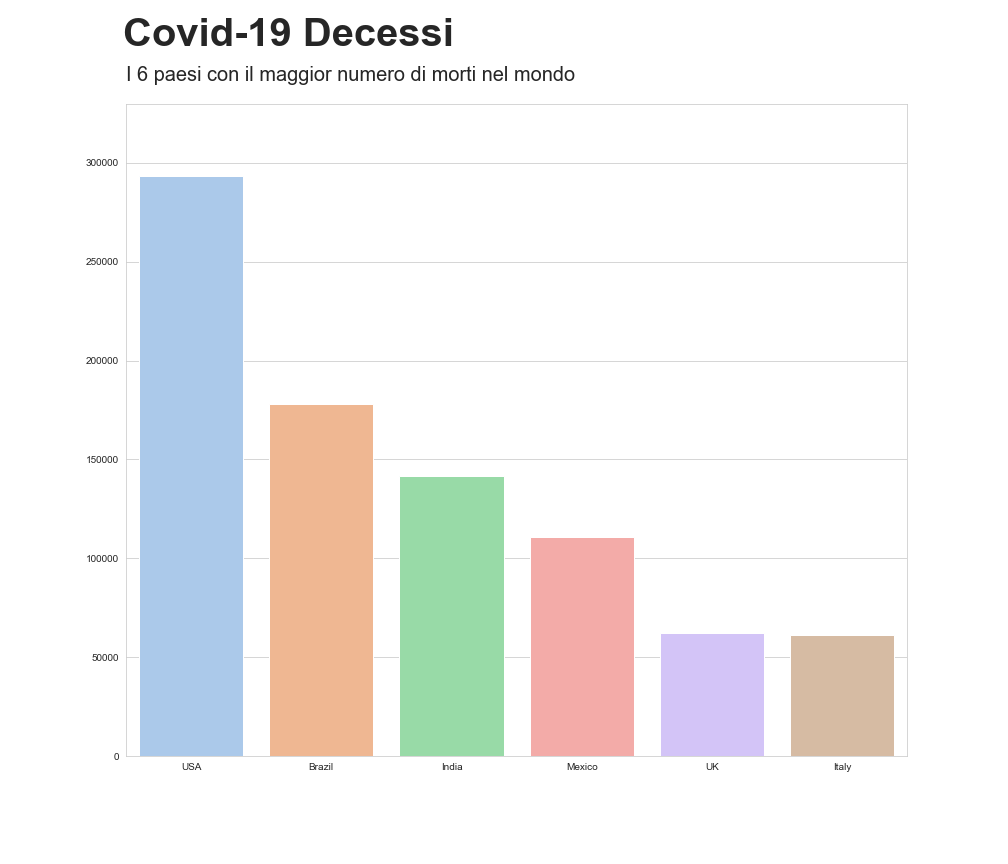
\includegraphics[scale=0.4]{Pictures/graph1}
%\caption{Come includere una figura, salvata nella cartella immagini.}\label{fig:figura2}
%\end{figure}




\chapter{Algoritmi predittivi}

\section{Algoritmo di Itti}

Presentiamo adesso un modello sull'attenzione visiva che si ispira al comportamento dell'architettura neurale proposta dai primi sistemi visivi. In particolare Itti ha basato il suo studio della salienza sul movimento dell'occhio dalla teoria delle \textit{feature maps} di Triesman. Più caratteristiche grafiche sono combinate in un'unica \textit{saliceny map} con scale diverse e successivamente un \textit{neural network} dinamico seleziona le zone in ordine di salienza decrescente. 

Il modello è basato sulla teoria dell'integrazione delle caratteristiche, la quale descrive le strategie e le metodologie  adottate nella ricerca visiva umana. L'input visivo, cioè l'immagine che l'osservatore sta fissando, è prima decomposto in un insieme di \texit{feature maps}. Zone differenti dell'immagine competono per la salienza e solo quelle che si distinguono rispetto alle altre sopravvivono ad una prima scrematura. Tutte queste mappe confluiscono poi in un'unica \textit{saliency map} mediante delle semplici combinazioni lineari.
Entrando più nel vivo, data in ingresso un'immagine a colori, vengono generati 9 valori di scala utilizzando la piramide gaussiana che progressivamente sottocampiona sempre di più l'immagine. Ogni proprietà visiva è poi calcolata mediante un insieme di operazioni lineari che legano il centro dell'immagine con ciò che c'è intorno. Per i colori, sull'immagine in ingresso vengono utilizzati i canali RGB (\textit{red}, \textit{green} e \textit{blue}) che forniscono un'intensità dell'immagine semplicemente come una media tra loro tre. Questa è usata per creare le piramidi gaussiane con i vari valori di scala. Il primo insieme di  \texit{feature maps} è costruito concentrandosi sul contrasto e quindi dove c'è una discrepanza tra la luminosità nel centro e sul bordo. Un secondo insieme di \texit{feature maps} è invece realizzato partendo dai canali dei colori. Infine l'ultimo gruppo è calcolato sulla base dell'orientazione usando le piramidi di Gabor orientate, nelle quali si combinano sia i valori di scala e sia alcuni valori per angoli di rotazione. Alla fine di questa prima parte ci saranno in tutto 42  \texit{feature maps}: 6 per l'intensità, 12 per i colori e 24 per l'orientazione. 

Il passo successivo è quello di costruire la mappa di salienza e quindi di associare ad ogni zona dell'immagine un valore scalare che rappresenti quanto questa è potenzialmente rilevante. Come prima cosa viene effettuata una combinazione delle \texit{feature maps} che è un input della mappa di salienza, modellata come un \textit{neural network} dinamico. Una delle difficoltà nel combinare insieme questi elementi è ad esempio che alcune sono difficili da confrontare tra di loro e gli elementi salienti appaiono rilevanti solo in poche di queste e quindi rischiano di perdersi una volta che vengono combinate tutte insieme. Per ovviare a questo problema è stato inserito un operatore di normalizzazione per ogni caratteristica e tre sono le mappe calcolate: una per l'intensità, una per il colore e una per l'orientazione. Queste sono poi normalizzate e ne viene fatta la media per ottenere la \textit{saliency map} finale. In ogni istante, il valore massimo della mappa di salienza identifica la regione dell'immagine più saliente verso la quale l'attenzione di chi guarda dovrebbe essere diretta.  

Il modello proposto ha un'architettura relativamente semplice, ma nonostante questo è in grado di fornire buone prestazioni con anche scene complesse riferite a situazioni naturali (quindi tipo fotografie di paesaggi o luoghi reali) e questo rinforza l'idea che un'unica mappa di salienza che riceve input dalle prime elaborazioni del processo visivo sia sufficiente per il processo \textit{bottom up}. Da un punto di vista computazionale la forza di questo approccio è la parallelizzazione delle varie caratteristiche visive, ma un difetto è la difficoltà di rilevare come salienti degli oggetti presentano una combinazione di più caratteristiche visive. Una componente cruciale del modello è la normalizzazione, la quale fornisce un meccanismo generico per calcolare la salienza in qualunque situazione. 

Altri modelli di questo tipo che verranno brevemente citati nella sezione successiva sono il BMS (\textit{Boolean Map Based Saliency model}) e l'eDN (\textit{Ensembles of Deep Networks Model}).

I grafici di business, o in generale i grafici di dati (che sono quelli che interessano a noi) non hanno però le stesse caratteristiche delle immagini che ritraggono situazioni del mondo reale. Quindi nella sezione successiva evidenziamo le problematiche e presenteremo la soluzione proposta da Matzen che abbiamo adottato per i nostri scopi durante questo lavoro di tesi.



\section{Algoritmo di Matzen}

I modelli che determinano la saliency visiva (ad esempio Itti) sono tipicamente basati sulle proprietà della corteccia visiva umana e predicono quali aree di un'immagine hanno delle caratteristiche visive tali da attirare l'attenzione dell'osservatore. Questi modelli tipicamente possono predirre abbastanza bene dove gli osservatori guarderanno in immagini di tipo naturale (quindi fotografie di situazioni reali), ma le loro prestazioni calano in visualizzazioni astratte, quindi per quanto riguarda ad esempio grafici di dati. In questa sezione discuteremo i motivi di questo calo ed è presentata la prima soluzione proposta, ovvero l'algoritmo di Matzen. 

Nel contesto di grafici di dati, le caratteristiche visive e la loro disposizione sull'immagine sono scelte per un particolare obiettivo. Chi crea i grafici, struttura l'immagine per comunicare informazioni in maniera tale che chi sta guardando possa trovare ciò che sta cercando in maniera agile. Oltretutto a differenza delle immagini naturali, i grafici di business sono tipicamente di origine digitale, quindi generati da computer ed è più facile isolare alcune zone della figura come ad esempio degli specifici gruppi di dati oppure delle porzioni di testo. 

I modelli sulla saliency visiva che inizialmente Matzen ha preso come riferimento sono stati Itti, eDN e BMS. Tutti seguono un approccio comune in cui come prima cosa vengono calcolate delle mappe di interesse a varie risoluzioni e successivamente vengono combinate insieme per costituire la mappa di salienza. Questa strategia funziona bene per immagini naturali, ma nella visualizzazione di dati le proprietà spaziali sono diverse: alcuni elementi (linee o porzioni di testo) sono piccoli e nel processo di sottocampionamento si rischia di perdere alcuni dettagli. Ad esempio con ciascuno dei modelli appena citati, il testo diventa sfocato e perde il suo significato nel corso delle analisi. Un'altra problematica di questi algoritmi già esistenti è che spesso come primo step viene effettuato un riscalamento dell'immagine ad una dimensione standard e questo può essere grave perchè porta certi elementi grafici a deformarsi e quindi a perdere le loro proprietà. Un altro aspetto su cui concentrarsi è quello dei colori. La percezione umana del colore è differente tra colori su carta oppure su un display elettronico e quindi la modifica proposta è stata quella di lavorare con lo spazio dei colori \textit{CIE LAB} che utilizza tre canali: due di colore e uno per la luminosità dell'immagine.  Una differenza cruciale tra grafici di dati e le immagini naturali è costituita sicuramente dalla presenza di grandi spazi bianchi (tipicamente) in cui sostanzialmente non ci sono informazioni da rilevare. L'aspetto però più rilevante di tutti è senza dubbio quello del testo. Questo in generale non è presente (oppure se sì in quantità limitata) nelle immagini naturali, mentre costituisce un elemento importante nei grafici di dati per trasmettere informazioni. Da ricerche che sono state effettuate, più del 60\% dell'attenzione ricade esclusivamente su parti scritte, a discapito di zone contenenti parti puramente grafiche. Dato che, come già scritto in precedenza, nei primi modelli di saliency citati il testo nel corso dell'analisi diventa sfocato, è stato necessario introdurre una parte dell'algoritmo che si concentrasse esclusivamente su di esso.

Il nuovo modello di saliency presentato per i grafici di dati, chiamato modello DVS (\textit{Data Visualization Saliency}),  è costituito da due parti principali: la prima è una versione modificata del modello di Itti e la seconda si occupa di riconoscere il testo.
\begin{figure}[!htb]\centering
\begin{subfigure}
\centering
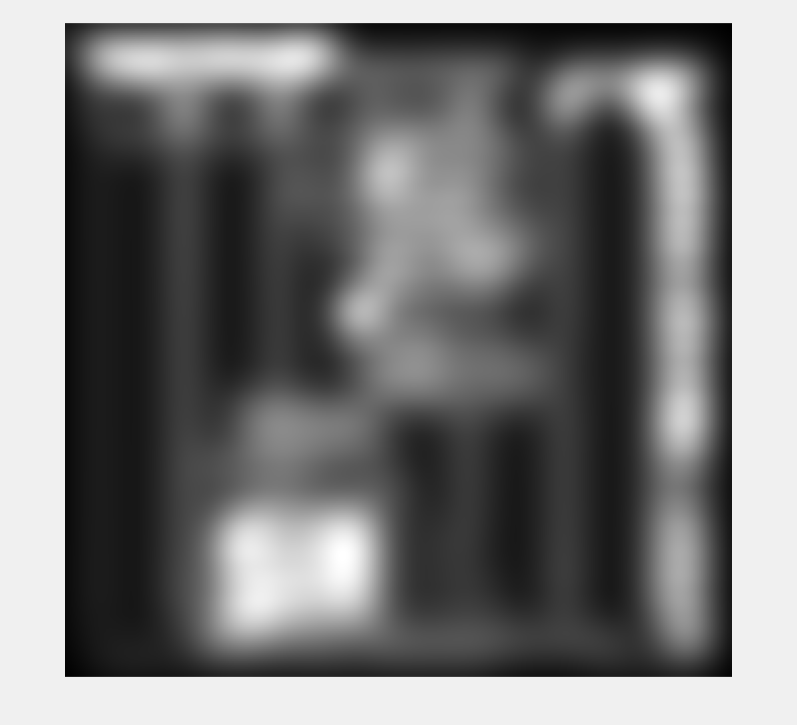
\includegraphics[scale=0.3]{CARICAMENTI_TESI/Caricamento_1_25_ottobre_2020/1_caricamento_25_ottobre_2020/immagini_algoritmo/economist_daily_chart_4/ITTI_OR_economist_daily_chart_4}
\end{subfigure}
\begin{subfigure}
\centering
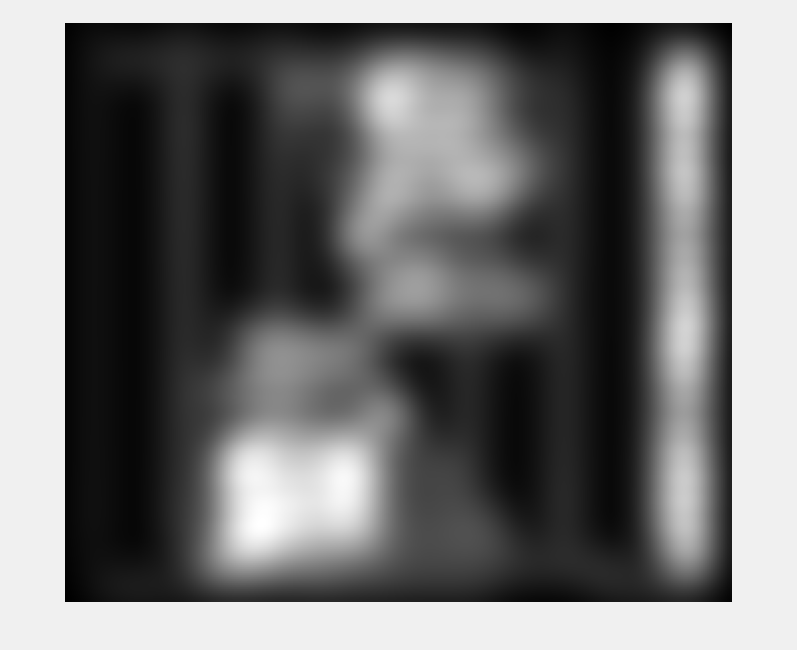
\includegraphics[scale=0.3]{CARICAMENTI_TESI/Caricamento_1_25_ottobre_2020/1_caricamento_25_ottobre_2020/immagini_algoritmo/economist_daily_chart_4/ITTI_economist_daily_chart_4}
\end{subfigure}
\begin{subfigure}
\centering
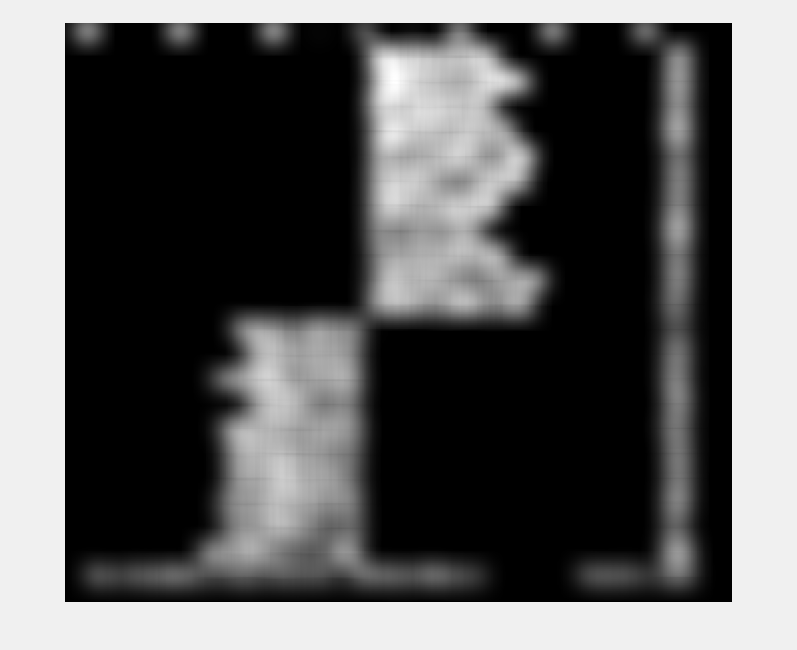
\includegraphics[scale=0.3]{CARICAMENTI_TESI/Caricamento_1_25_ottobre_2020/1_caricamento_25_ottobre_2020/immagini_algoritmo/economist_daily_chart_4/TextSaliency_economist_daily_chart_4}
\end{subfigure}
\begin{subfigure}
\centering
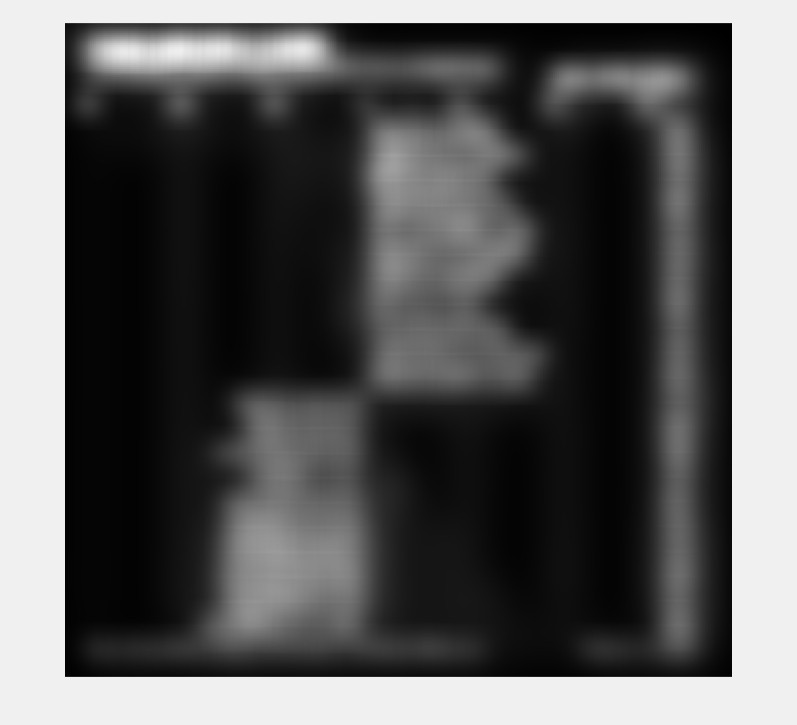
\includegraphics[scale=0.3]{CARICAMENTI_TESI/Caricamento_1_25_ottobre_2020/1_caricamento_25_ottobre_2020/immagini_algoritmo/economist_daily_chart_4/Combination_economist_daily_chart_4}
\end{subfigure}
\caption{Analisi algoritmo Matzen}\label{fig: Combination_economist_daily_chart_4}
\end{figure}
Come primo riferimento di partenza, è stato preso Itti perchè sul dataset \texit{MASSVIS} sul quale si stava lavorando (che è descritto nella sezione successiva) è il modello sulla saliency visiva con le migliori prestazioni (in relazione ad 8 metriche anche queste descritte nella prossima sezione). 
La modifica effettuata riguarda i colori. Itti originale utilizza il riconoscimento dei colori tramite i canali RGB, ma dato che non trattiamo più immagini naturali e i colori possono essere scelti liberamente da chi crea i grafici, è bene cambiare la metodologia con la quale i colori vengono analizzati. Per questo il modello è stato modificato, trasformando la rappresentazione delle immagini in input tramite lo spazio dei colori \textit{CIE LAB}.
Nella parte superiore della figura \ref{fig: Combination_economist_daily_chart_4} sono messi a confronto i risultati prodotti dalle analisi di Itti originale (a sinistra) e Itti modificato (a destra) sulla prima immagine in figura \ref{fig: economist_daily_chart_4} del dataset di \texit{MASSVIS}. Come si può notare, il cambiamento a livello visivo non è eclatante, infatti la modifica si risente maggiormente a livello di prestazioni numeriche delle metriche su questo tipo di immagini, in particolare quando Itti modificato (che a livello grafico produce una mappa meno sfocata) viene combinato insieme all'analisi del testo. 

Come già accennato in precedenza, gli osservatori dedicano la maggior parte dell'attenzione nei confronti del testo nei grafici di dati. Spesso queste porzioni tendono ad avere un elevato contrasto e ad essere piccole. In più l'elevata frequenza in queste zone tende ad essere persa quando si effettuano dei riscalamenti. A tal proposito Matzen ha realizzato una porzione del modello che si occupa di riconoscere esclusivamente il testo per poi poter essere combinata con Itti modificato. Il metodo utilizzato per questo scopo è una combinazione di varie tecniche classiche di riconoscimento del testo già esistenti. A differenza di queste però, non viene prodotto un output binario (testo c'è/testo non c'è) bensì viene generata una distribuzione continua di probabilità che può essere incorporata ad una \textit{saliency map}. Più nel dettaglio l'approccio utilizzato è stato l'MSER (\textit{Maximally Stable Extremal Regions}). Con questo algoritmo si cercano delle regioni che sono possibili candidate a contenere del testo (regioni di pixel omogenee e connesse), per poi applicare su queste alcuni indicatori del testo che fanno da filtro e permettono di escludere chi non ne contiene. In basso a sinistra in figura \ref{fig: Combination_economist_daily_chart_4} c'è il risultato dell'analisi sul testo della prima immagine in figura \ref{fig: economist_daily_chart_4} e possiamo notare come tutto il testo venga correttamente identificato.

Infine quello che Matzen ha eseguito è stata una combinazione lineare tra Itti modificato e l'analisi sul testo per generare la sua mappa di salienza. Nel complesso questa produce sulle metriche (con cui vengono misurate le prestazioni) risultati migliori rispetto ai precedenti algoritmi. Nel documento [3] si trovano le tabelle numeriche riassuntive che dimostrano la superiorità dell'algoritmo di Matzen per quanto riguarda il dataset fornito da \textit{MASSVIS}. Nelle sezioni seguenti andremo anche noi a verificare queste informazioni per cercare se è presente qualche difetto e se si è in grado si proporre qualcosa di migliore o di competitivo. Nella parte in basso a destra di figura \ref{fig: Combination_economist_daily_chart_4} è mostrata la combinazione tra Itti modificato (in alto a destra) e l'analisi sul testo (in basso a sinistra) della prima immagine in figura \ref{fig: economist_daily_chart_4} del dataset di \textit{MASSVIS} (descritto nella pagina successiva). Come emergerà anche successivamente dall'esperimento da noi creato, quando il testo è presente in maniera prepotente sull'immagine attira quasi tutta l'attenzione. Ad esempio, anche per questa mappa di salienza combinata, ciò di cui rimane traccia è per lo più il testo e la parte grafica (quindi le barre) praticamente non è evidenziata.



\section{Dataset e verifiche}
Come già espresso nella sezione precedente, il lavoro di Matzen si è concentrato su analizzare i dati forniti da \href{http://massvis.mit.edu}{\textit{MASSVIS}} e qui entriamo più nel dettaglio dei risultati da lei ottenuti (che abbiamo replicato). \textit{MASSVIS} è un dataset per la visualizzazione di immagini raffiguranti grafici di dati e le cui fonti sono i dati messi a disposizione dai governi, i grafici informativi, le notizie e la scienza.

\begin{figure}[!htb]\centering
\begin{subfigure}
\centering
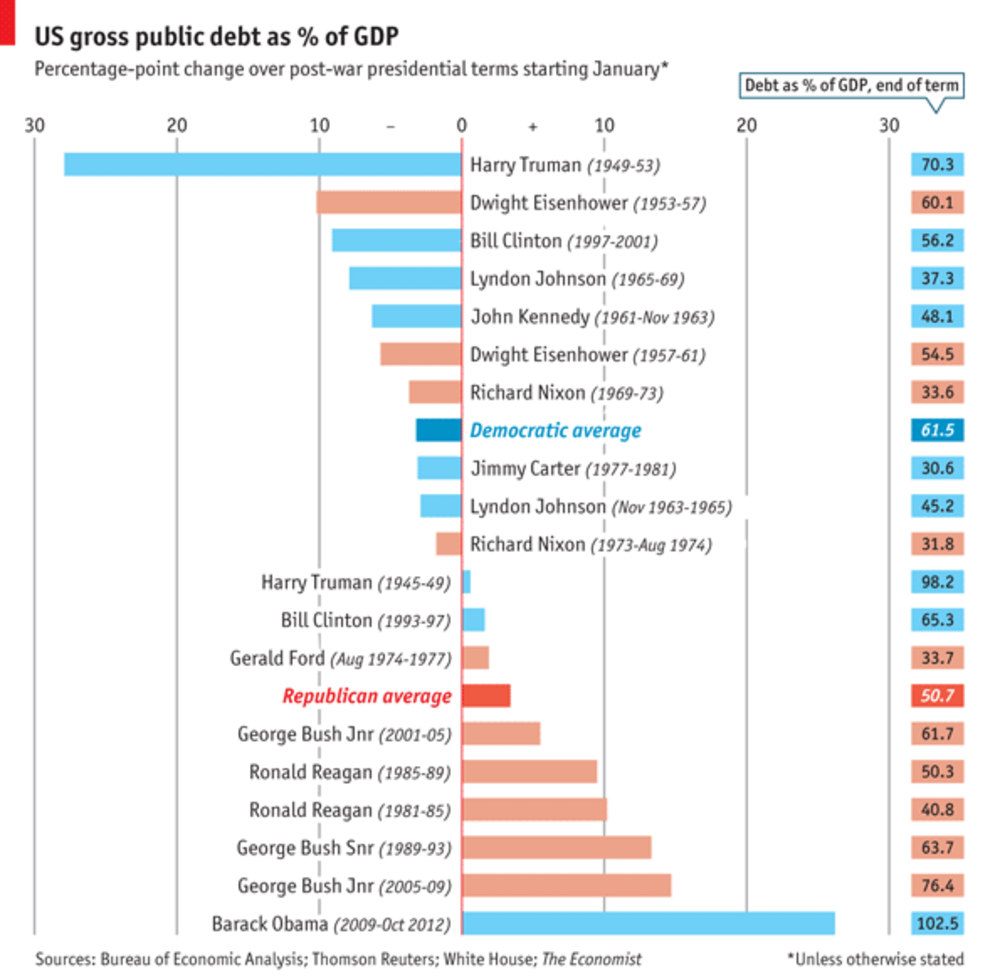
\includegraphics[scale=0.2]{CARICAMENTI_TESI/Caricamento_1_25_ottobre_2020/1_caricamento_25_ottobre_2020/immagini_originali/economist_daily_chart_4}
\end{subfigure}
\begin{subfigure}
\centering
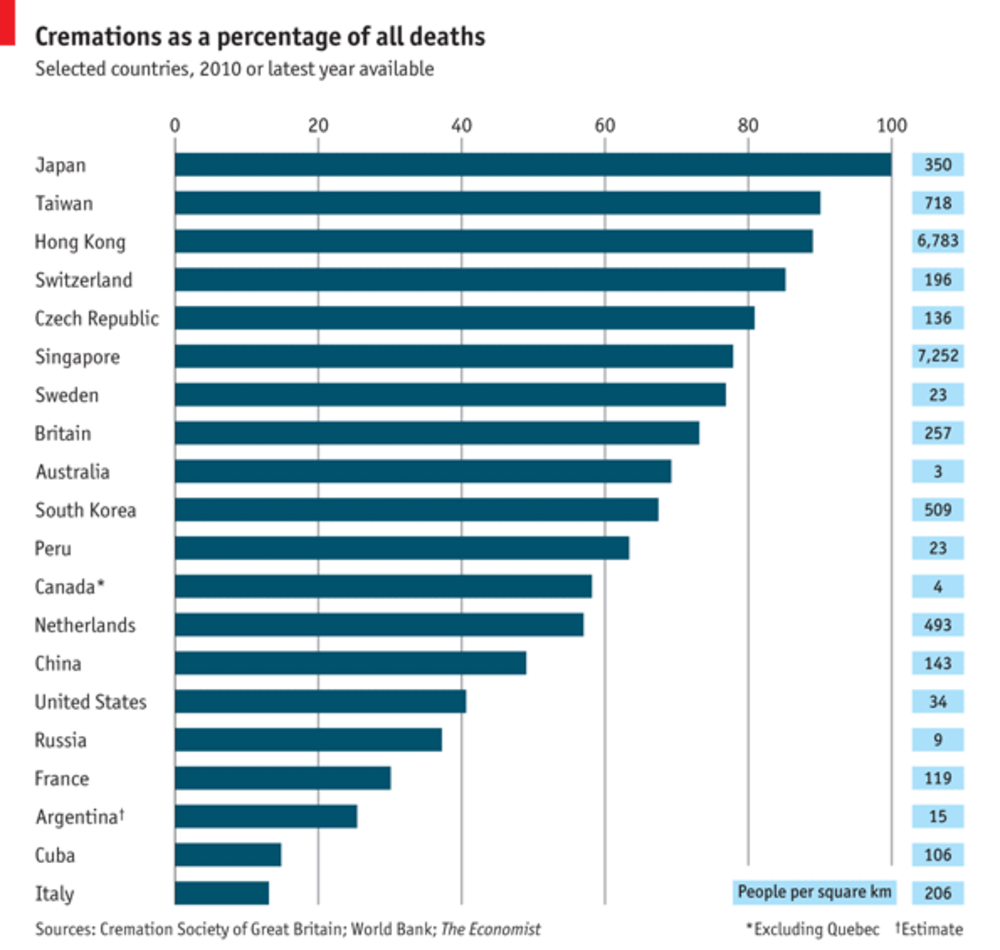
\includegraphics[scale=0.2]{CARICAMENTI_TESI/Caricamento_1_25_ottobre_2020/1_caricamento_25_ottobre_2020/immagini_originali/economist_daily_chart_5}
\end{subfigure}
\begin{subfigure}
\centering
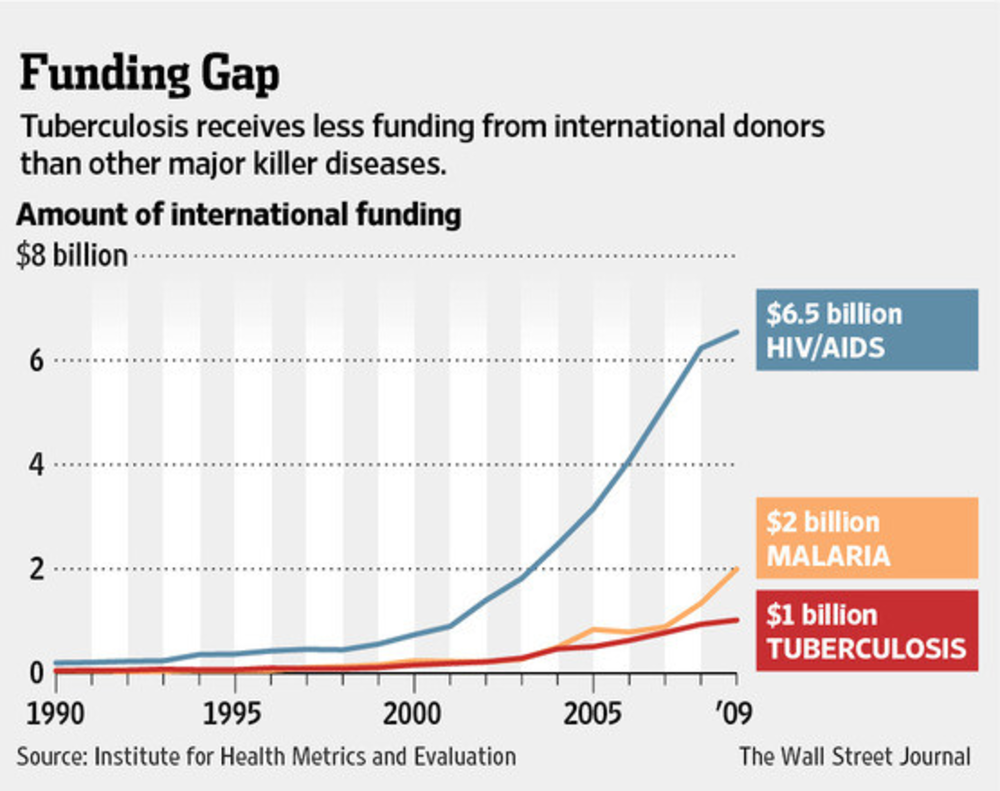
\includegraphics[scale=0.2]{CARICAMENTI_TESI/Caricamento_1_25_ottobre_2020/1_caricamento_25_ottobre_2020/immagini_originali/wsj612}
\end{subfigure}
\begin{subfigure}
\centering
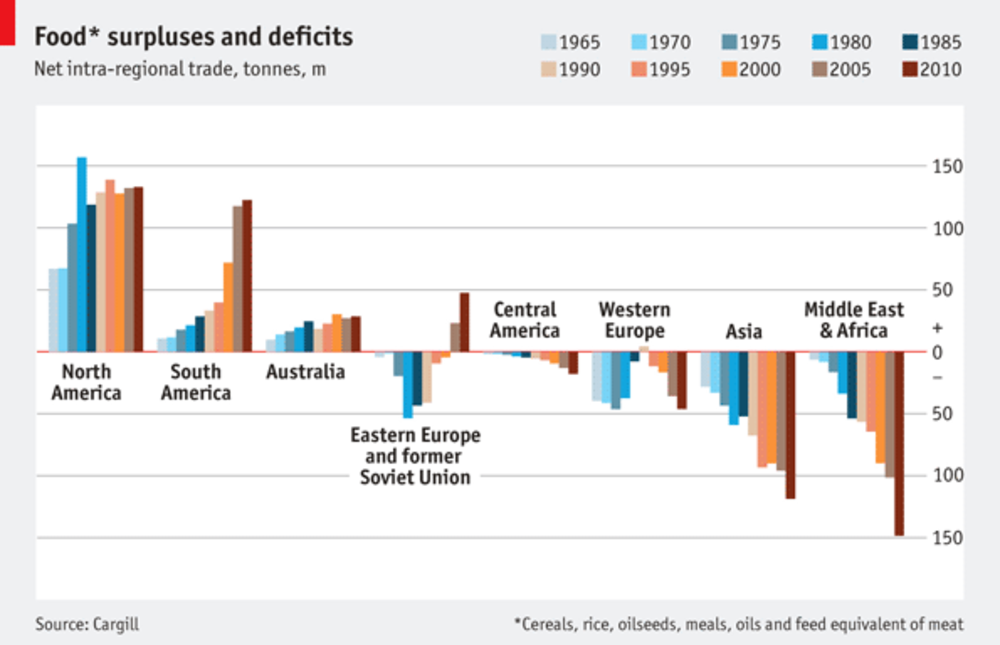
\includegraphics[scale=0.2]{CARICAMENTI_TESI/Caricamento_1_25_ottobre_2020/1_caricamento_25_ottobre_2020/immagini_originali/economist_daily_chart_103}
\end{subfigure}
\caption{Dataset MASSVIS}\label{fig: economist_daily_chart_4}
\end{figure}

%\begin{figure}[!htb]\centering
%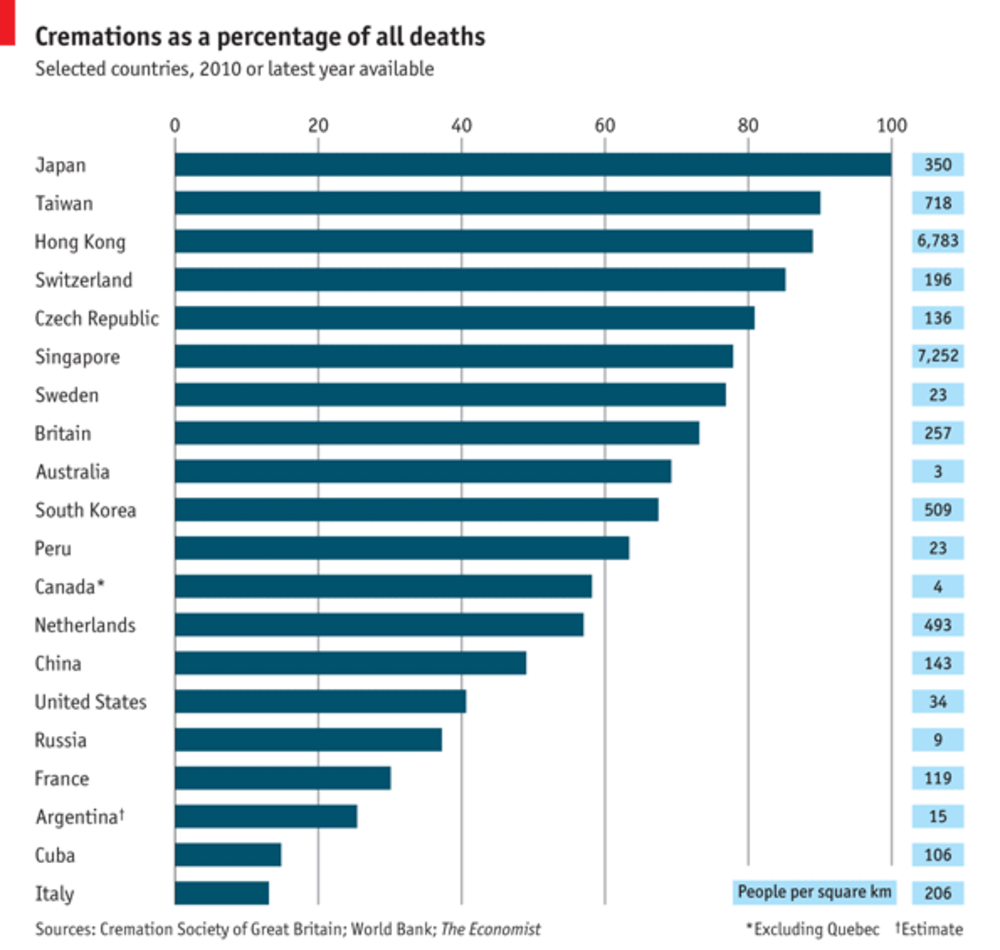
\includegraphics[scale=0.5]{CARICAMENTI_TESI/Caricamento_1_25_ottobre_2020/1_caricamento_25_ottobre_2020/immagini_originali/economist_daily_chart_5}
%\caption{...}\label{fig: economist_daily_chart_5}
%\end{figure}

%\begin{figure}[!htb]\centering
%\includegraphics[scale=0.6]{CARICAMENTI_TESI/Caricamento_1_25_ottobre_2020/1_caricamento_25_ottobre_2020/immagini_algoritmo/economist_daily_chart_4/Final_economist_daily_chart_4}
%\caption{...}\label{fig: Final_economist_daily_chart_4}
%\end{figure}

Nel link al dataset (indicato in blu) è presente una sezione che si chiama \textit{Eye-movement Data} in cui ci viene descritto l'esperimento di eye tracking che è stato eseguito per raccogliere i dati. Il dataset è composto da 393 immagini (di vario genere) che sono state mostrate per 10 secondi a 33 osservatori dei quali si è tracciato il movimento dell'occhio. Ogni immagine è stata vista da almeno 16 osservatori. 

In figura \ref{fig: economist_daily_chart_4} sono rappresentate quattro immagini presenti in \text{MASSVIS} per dare un'idea di quali tipologie di grafici si sta parlando. Rispettivamente i nomi di queste sono: \textit{economist\_daily\_chart\_4}, , \textit{economist\_daily\_chart\_5}, \textit{economist\_daily\_chart\_103} e \textit{wsj612}. 
\begin{figure}[!htb]\centering
\begin{subfigure}
\centering
\includegraphics[scale=0.3]{CARICAMENTI_TESI/Caricamento_1_25_ottobre_2020/1_caricamento_25_ottobre_2020/immagini_algoritmo/economist_daily_chart_4/EyeTracking_economist_daily_chart_4}
\end{subfigure}
\begin{subfigure}
\centering
\includegraphics[scale=0.3]{CARICAMENTI_TESI/Caricamento_1_25_ottobre_2020/1_caricamento_25_ottobre_2020/immagini_algoritmo/economist_daily_chart_4/Final_economist_daily_chart_4}
\end{subfigure}
\begin{subfigure}
\centering
\includegraphics[scale=0.3]{CARICAMENTI_TESI/Caricamento_1_25_ottobre_2020/1_caricamento_25_ottobre_2020/immagini_algoritmo/economist_daily_chart_5/EyeTracking_economist_daily_chart_5}
\end{subfigure}
\begin{subfigure}
\centering
\includegraphics[scale=0.3]{CARICAMENTI_TESI/Caricamento_1_25_ottobre_2020/1_caricamento_25_ottobre_2020/immagini_algoritmo/economist_daily_chart_5/Final_economist_daily_chart_5}
\end{subfigure}
\caption{Confronto punti di fissazione e Matzen}\label{fig: EyeTracking_economist_daily_chart_4}
\end{figure}
Precisiamo che delle 393 immagini presenti nel dataset, ne abbiamo conservate 110 in quanto alcune avevano sfondi troppo elaborati oppure non erano dei veri e propri grafici di dati e quindi non erano di nostro interesse. Nella sezione 4.3 di questo documento viene descritto tutto il materiale che abbiamo elaborato durante questi mesi di lavoro alla tesi e ci sono anche le informazioni su quali parti di \textit{MASSVIS} abbiamo conservato.

Scaricando il materiale \textit{Data} e il codice Matlab \textit{Code} dal sito di \textit{MASSVIS}  abbiamo potuto riprodurre le mappe di calore della saliency su ognuna delle immagini e confrontare quanto ottenuto con quello che l'algoritmo di Matzen genera.

Nelle figure \ref{fig: EyeTracking_economist_daily_chart_4} e \ref{fig: EyeTracking_economist_daily_chart_103} sono mostrate: a sinistra l'immagine originale di \textit{MASSVIS} alla quale è stata sovrapposta la mappa di calore in seguito ai dati analizzati dall'eye tracking e a destra la saliency che viene prodotta da Matzen per quell'immagine.

\begin{figure}[!htb]\centering
\begin{subfigure}
\centering
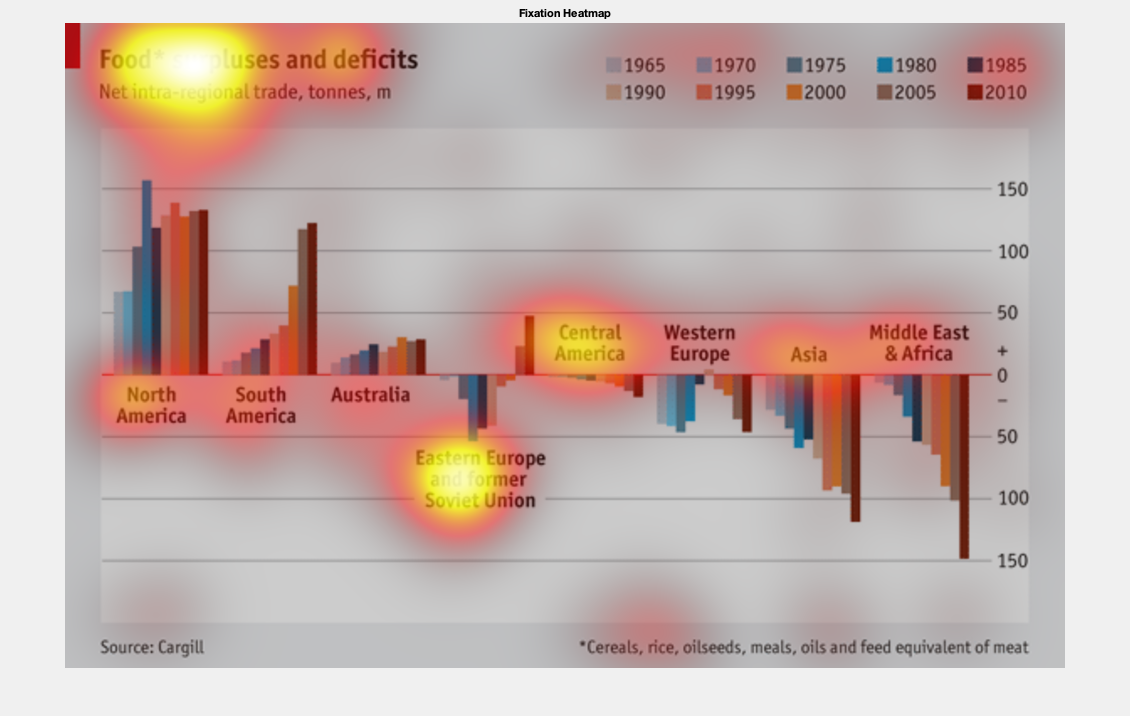
\includegraphics[scale=0.21]{CARICAMENTI_TESI/Caricamento_1_25_ottobre_2020/1_caricamento_25_ottobre_2020/immagini_algoritmo/economist_daily_chart_103/EyeTracking_economist_daily_chart_103}
\end{subfigure}
\begin{subfigure}
\centering
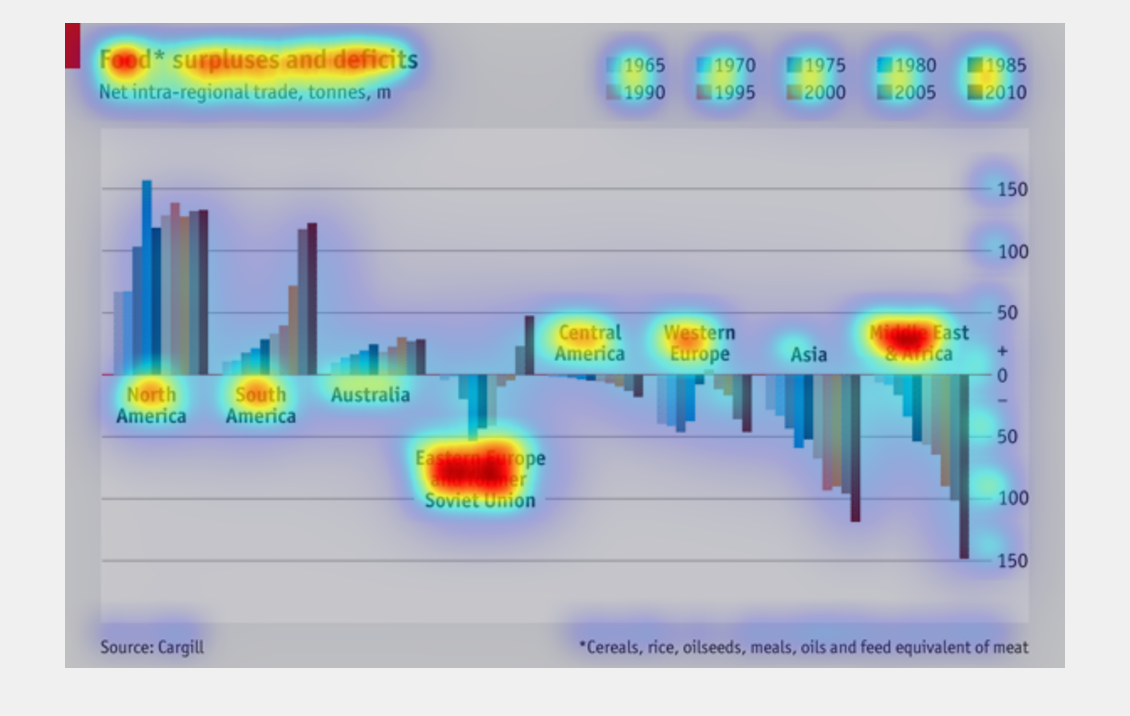
\includegraphics[scale=0.21]{CARICAMENTI_TESI/Caricamento_1_25_ottobre_2020/1_caricamento_25_ottobre_2020/immagini_algoritmo/economist_daily_chart_103/Final_economist_daily_chart_103}
\end{subfigure}
\begin{subfigure}
\centering
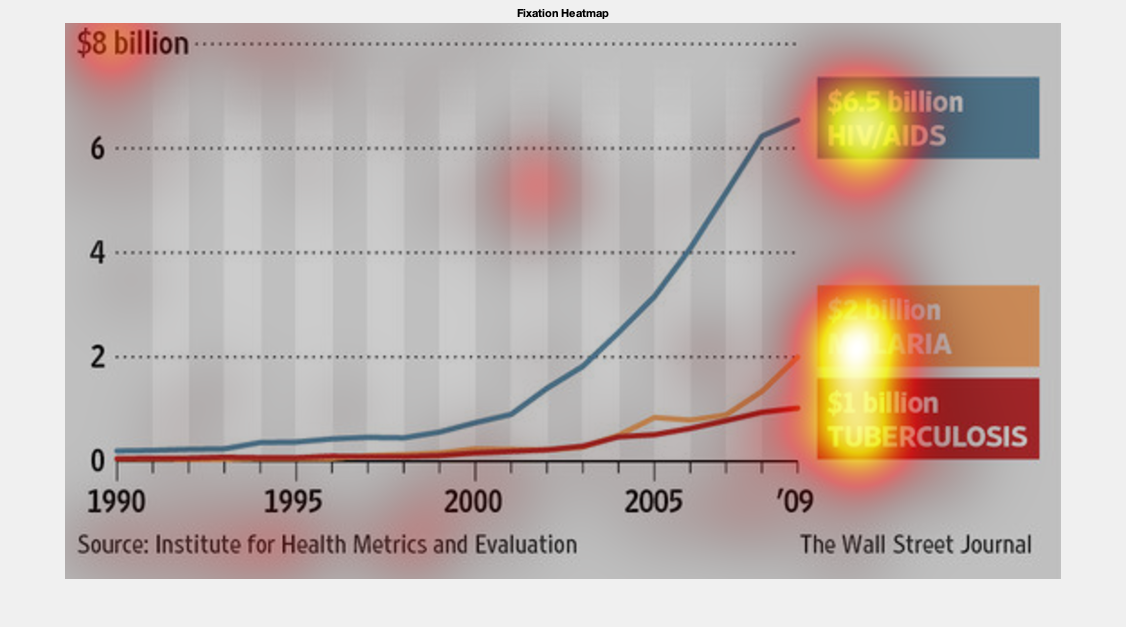
\includegraphics[scale=0.3]{CARICAMENTI_TESI/Caricamento_1_25_ottobre_2020/1_caricamento_25_ottobre_2020/immagini_algoritmo/wsj612/EyeTracking_wsj612}
\end{subfigure}
\begin{subfigure}
\centering
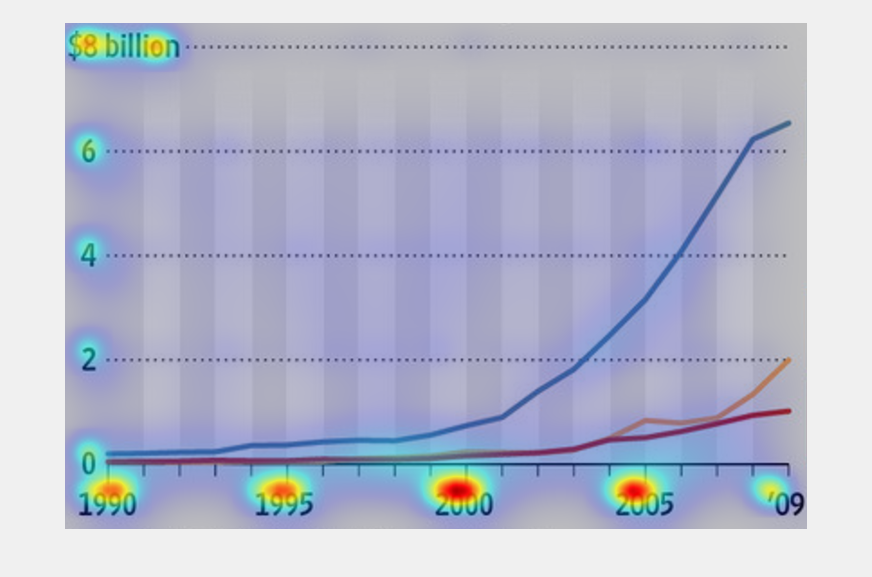
\includegraphics[scale=0.3]{CARICAMENTI_TESI/Caricamento_1_25_ottobre_2020/1_caricamento_25_ottobre_2020/immagini_algoritmo/wsj612/Final_wsj612}
\end{subfigure}
\caption{Confronto punti di fissazione e Matzen}\label{fig: EyeTracking_economist_daily_chart_103}
\end{figure}

Entreremo meglio nel merito di quanto graficamente viene mostrato, ma a primo impatto possiamo notare come la parte di testo presente sull'immagine (titolo, sottotiolo, legenda oppure etichetta dei dati) attiri la maggior parte dell'attenzione su di essa mentre le parti puramente grafiche sembrano essere un pò trascurate e lasciate in secondo piano.

Valutare le prestazioni di Matzen solo da un punto di vista grafico non è però sufficiente. Anche a livello numerico è bene quantificare le sue prestazioni in base a quanto la mappa di salienza che produce si discosta da quella vera generata dai dati raccolti sugli osservatori. A tal proposito, per questo tipo di calcoli sono disponibili 8 \href{http://saliency.mit.edu/results_mit300.html}{metriche} che abbiamo utilizzato:  le prime 3 si occupano di quantificare quanto bene la mappa di salienza di Matzen predice le zone in cui l'occhio umano si è realmente concentrato; le successive 4 eseguono una comparazione tra la distribuzione delle fissazioni sull'immagine e la distribuzione della salienza nella \textit{saliency map} dell'algoritmo; l'ultima esegue un'analisi un pò diversa descritta qui sotto. Le metriche sono elencate di seguito:
\begin{itemize}
\item \textit{AUC-Borji}: questa metrica misura quanto la mappa di salienza generata su un'immagine predice correttamente le regioni di fissazione dell'occhio umano;
\item \textit{AUC-Judd}: il compito di questa metrica è lo stesso della precedente, ma cambia come sono gestite le curve ROC (\textit{Receiver operating characteristic}) e la gestione dei falsi positivi; 
\item \textit{AUC-Shuffled}: anche lei ha lo stesso compito delle due metriche precedenti, ma cambia ancora come sono gestite le curve ROC (\textit{Receiver operating characteristic}) e la gestione dei falsi positivi; 
\item \textit{CC}: questa metrica calcola il coefficiente di correlazione lineare secondo Pearson tra due differenti mappe di salienza dove falsi negativi e falsi positivi sono penalizzati equamente; 
\item \textit{EMD}: questa metrica calcola il coefficiente denominato \textit{emd\_hat} descritto nel paper \textit{A Linear Time Histogram Metric for Improved SIFT Matching}. In particolare questo coefficiente rappresenta il costo di trasformare una mappa nell'altra, quindi più è alto e più significa che abbiamo ottenuto un risultato peggiore;
\item \textit{KL}: questa metrica trova la divergenza secondo Kullback e Leibler tra due differenti mappe di salienza quando sono viste come distribuzioni. Fornisce un'informazione di quanta informazione perdiamo quando la mappa di salienza dell'algoritmo è usata al posto di quella vera creata dai dati raccolti sugli osservatori. Come per la metrica precedente, anche per questa quando otteniamo il numero più alto significa che l'algoritmo ha performato peggio;
\item \textit{SIM}: questa metrica tratta le fissazioni e la mappa di salienza come istogrammi e calcola quanto si sovrappongono bene l'una sull'altra;
\item \textit{NSS}: questa metrica trova il \textit{saliency scanpath} normalizzato tra due differenti mappe di salienza. Standardizza la mappa di salienza dell'algoritmo e poi calcola la \textit{saliency} media in posizioni predefinite;
\end{itemize}

Servendoci delle metriche appena descritte e dei loro rispettivi codici Matlab abbiamo costruito la tabella \ref{t:1}. In essa sono riassunti i risultati per ognuna delle otto metriche dei tre algoritmi. In particolare la tabella è divisa in tre sezioni in maniera tale che siano confrontati tra di loro due algoritmi alla volta in termini di percentuale di vittorie su ognuna delle metriche. Rispettivamente nella prima sezione abbiamo le percentuali di vittorie tra Itti originale (\textit{ITTI OR}) e Itti modificato (\textit{ITTI MOD}), nella seconda c'è il confronto tra Matzen (\textit{MATZEN}) Itti originale e nella terza abbiamo Matzen comparato con Itti modificato.
%\begin{tiny}
\begin{table}[!htp] 
\small             
\centering                      
\begin{tabular} %{lllllll}   
%{c}               
{l c c c c c c c c}                  % parametri di incolonnamento: r (a destra), c (al centro), l (a sinistra),% p (per definire la larghezza della colonna)
\hline\hline
& AUC-Borji &  AUC-Judd &  AUC-S. &  CC &  EMD &  KL &  NSS &  SIM  \\  
\hline
%\hspace*{1.3em}
ITTI OR & 41,91\% & 37,27\% & 49,18\% & 50,91\% &  55,55\% & 65,55\%  & 41,91\% &  49,18\% \\
ITTI MOD & 59,09\% & 62,73\% & 51,82\% & 49,09\% & 45,45\%  & 35,45\%  & 59,09\% &  51,82\%\\
PAREGGIO & 0\% & 0\% & 0\% & 0\% & 0\% & 0\% & 0\% &  0\%\\
\hline \hline
& AUC-Borji &  AUC-Judd &  AUC-S. &  CC &  EMD &  KL &  NSS &  SIM  \\  
\hline
%\hspace*{1.3em}
MATZEN & 81,82\% & 97,27\% & 75,45\% & 90,90\% & 3,64\% & 0,91\% & 98,18\% & 85,45\% \\
ITTI OR & 19,18\% & 2,73\% & 25,55\% & 9,10\% & 96,26\% & 99,09\%  & 1,82\% &  13,64\%\\
PAREGGIO & 0\% & 0\% & 0\% & 0\% & 0\% & 0\% & 0\% & 0,91\%\\
\hline \hline
& AUC-Borji &  AUC-Judd &  AUC-S. &  CC &  EMD &  KL &  NSS &  SIM  \\  
\hline
%\hspace*{1.3em}
MATZEN & 82,73\% & 95,45\% & 80\% & 88,18\% & 3,64\%  & 4,55\% & 97,27\% & 86,36\% \\
ITTI MOD & 17,27\% & 4,55\% &   20\%  & 11,82\% & 96,26\% & 95,45\%  & 2,73\% &  13,64\%\\
PAREGGIO & 0\% & 0\% & 0\% & 0\% & 0\% & 0\% & 0\% &  0\%\\
\hline \hline
\end{tabular}
\caption[Risultati metriche globali MASSVIS]{Risultati metriche globali MASSVIS} \label{t:1}  
%[Short description for the content list.]{Complete descreption: caption of the table.}
\end{table}




Bisogna ricordarsi di tenere in considerazione il fatto che per le metriche \textit{EMD} e \textit{KL} i ragionamenti sono invertiti perchè vanno a misurare una dispersione rispetto alla vera mappa di salienza. 

Analizzando le percentuali in tabella abbiamo la conferma che Matzen sia effettivamente, almeno su queste immagini, l'algoritmo migliore tra i tre di cui stiamo discutendo. Nelle prossime sezioni cercheremo di trovare dei difetti a questo algoritmo e vedere se performa meglio degli altri due anche apportando delle piccole modifiche alle immagini che abbiamo conservato di \textit{MASSVIS}.

%\end{tiny}
%\begin{table}[htp]              
%\centering                      
%\begin{tabular} %{lllllll}   
%%{c}               
%{l c c c c c c c c}                  % parametri di incolonnamento: r (a destra), c (al centro), l (a sinistra), % p (per definire la larghezza della colonna)
%\hline\hline
%& AUC-Borji &  AUC-Judd &  AUC-Shuffled &  CC &  EMD &  KL &  NSS &  SIM  \\  
%\hline
%%\hspace*{1.3em}
%MATZEN & 81,82\% & 97,27\% & 75,45\% & 90,90\% & 3,64\% & 0,91\% & 98,18\% & 85,45\% \\
%ITTI OR & 19,18\% & 2,73\% & 25,55\% & 9,10\% & 96,26\% & 99,09\%  & 1,82\% &  13.64\%\\
%PAREGGIO & 0\% & 0\% & 0\% & 0\% & 0\% & 0\% & 0\% & 0,91\%\\
%\hline \hline
%\end{tabular}
%\caption[Descrizione breve: compare nell'elenco tabelle]{...(scrivi)...} \label{t:1}  
%%[Short description for the content list.]{Complete descreption: caption of the table.}
%\end{table}
%
%\begin{table}[H]              
%\centering                      
%\begin{tabular} %{lllllll}   
%%{c}               
%{l c c c c c c c c}                  % parametri di incolonnamento: r (a destra), c (al centro), l (a sinistra),	% p (per definire la larghezza della colonna)
%\hline\hline
%& AUC-Borji &  AUC-Judd &  AUC-Shuffled &  CC &  EMD &  KL &  NSS &  SIM  \\  
%\hline
%%\hspace*{1.3em}
%MATZEN & 82,73\% & 95,45\% & 80\% & 88,18\% & 3,64\%  & 4,55\% & 97,27\% & 86,36\% \\
%ITTI MOD & 17,27\% & 4,55\% &   20\%  & 11,82\% & 96,26\% & 95,45\%  & 2,73\% &  13,64\%\\
%PAREGGIO & 0\% & 0\% & 0\% & 0\% & 0\% & 0\% & 0\% &  0\%\\
%\hline \hline
%\end{tabular}
%\caption[Descrizione breve: compare nell'elenco tabelle]{...(scrivi)...} \label{t:1}  
%%[Short description for the content list.]{Complete descreption: caption of the table.}
%\end{table}

\section{Analisi semantica}
In questa sezione ci siamo concentrati sull'\textit{analisi semantica}, ovvero sulla distribuzione dei poligoni (forniti dal dataset) sull'immagine. Ogni poligono circonda una determinata porzione dell'immagine: ad esempio il titolo, il sottotitolo, altre porzioni scritte sull'immagine, la legenda oppure le parti puramente grafiche (andando in alcune più nel dettaglio e in altre un pò di meno). 
\begin{figure}[!htb]\centering
\begin{subfigure}
\centering
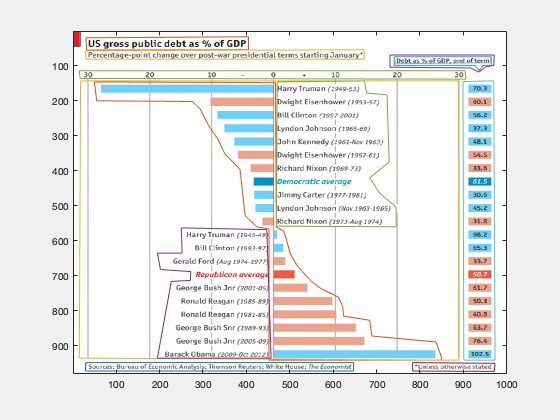
\includegraphics[scale=0.46]{CARICAMENTI_TESI/Caricamento_7_8_dicembre_2020/7_caricamento_8_dicembre_2020/analisi_semantica_immagini/economist_daily_chart_4/POLY_ON_IMG_economist_daily_chart_4}
\end{subfigure}
\begin{subfigure}
\centering
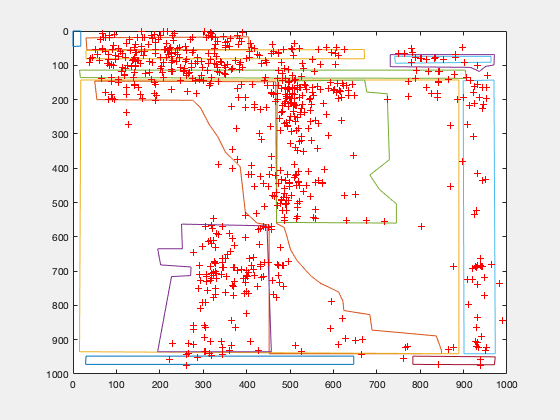
\includegraphics[scale=0.46]{CARICAMENTI_TESI/Caricamento_7_8_dicembre_2020/7_caricamento_8_dicembre_2020/analisi_semantica_immagini/economist_daily_chart_4/POLY_AND_POINTS_economist_daily_chart_4}
\end{subfigure}
\begin{subfigure}
\centering
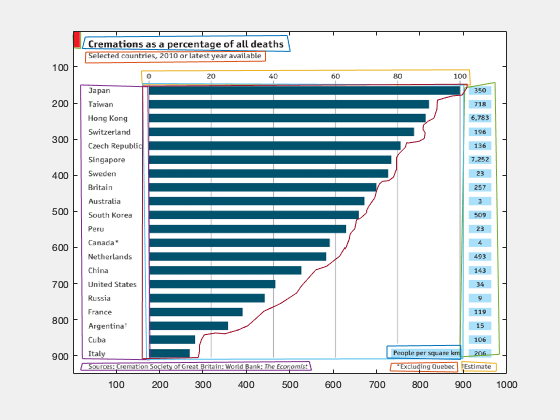
\includegraphics[scale=0.46]{CARICAMENTI_TESI/Caricamento_7_8_dicembre_2020/7_caricamento_8_dicembre_2020/analisi_semantica_immagini/economist_daily_chart_5/POLY_ON_IMG_economist_daily_chart_5}
\end{subfigure}
\begin{subfigure}
\centering
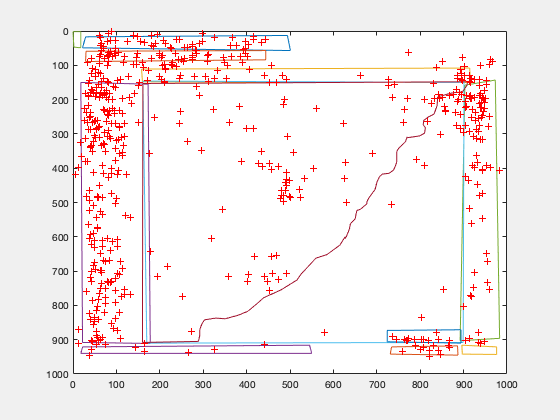
\includegraphics[scale=0.45]{CARICAMENTI_TESI/Caricamento_7_8_dicembre_2020/7_caricamento_8_dicembre_2020/analisi_semantica_immagini/economist_daily_chart_5/POLY_AND_POINTS_economist_daily_chart_5}
\end{subfigure}
\begin{subfigure}
\centering
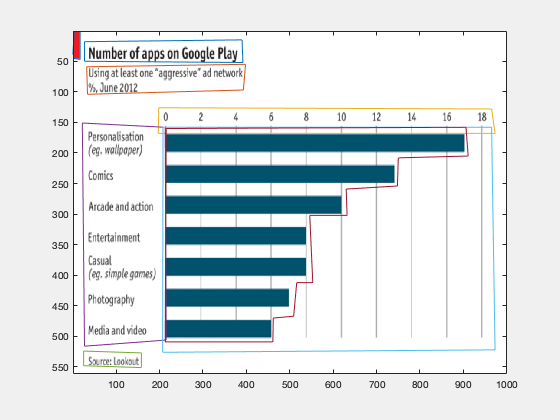
\includegraphics[scale=0.45]{CARICAMENTI_TESI/Caricamento_7_8_dicembre_2020/7_caricamento_8_dicembre_2020/analisi_semantica_immagini/economist_daily_chart_75/POLY_ON_IMG_economist_daily_chart_75}
\end{subfigure}
\begin{subfigure}
\centering
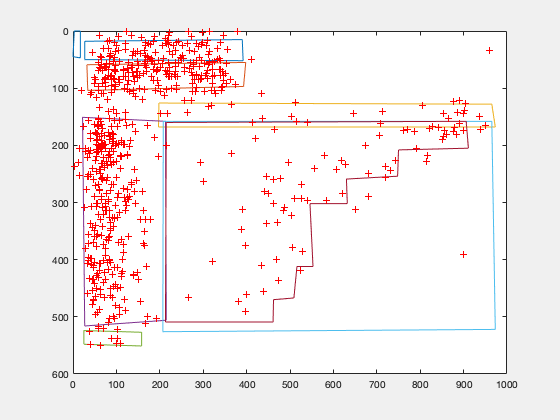
\includegraphics[scale=0.46]{CARICAMENTI_TESI/Caricamento_7_8_dicembre_2020/7_caricamento_8_dicembre_2020/analisi_semantica_immagini/economist_daily_chart_75/POLY_AND_POINTS_economist_daily_chart_75}
\end{subfigure}
\caption{Analisi semantica}\label{fig: POLY_ON_IMG_economist_daily_chart_4}
\end{figure}
Per essere più precisi il dataset \textit{MASSVIS} mette a disposizione un file di testo per ogni immagine e questo contiene le informazioni sui punti che delimitano ogni poligono. 


Lo scopo di questa analisi è come prima cosa mostrare come sono distribuiti questi poligoni sull'immagine. In seguito, alla luce di quanto era risultato dall'analisi nella sezione precedente, abbiamo rappresentato anche i punti di fissazione in una nuova immagine con sfondo bianco contenente solo i poligoni. In questa maniera siamo stati in grado di verificare anche graficamente che questi punti fossero maggiormente concentrati nelle zone contenenti del testo dato che fino ad ora non avevamo avuto informazioni sui singoli punti di fissazione, ma avevamo solo la mappa di calore dalla quale poter estrarre delle informazioni.

In figura \ref{fig: POLY_ON_IMG_economist_daily_chart_4} sono riportati i risultati grafici di tre immagini contenute in \texit{MASSVIS}, in particolare: \textit{economist\_daily\_chart\_4}, \textit{economist\_daily\_chart\_5} ed \textit{economist\_daily\_} \textit{chart\_75}. Come si può notare, a sinistra abbiamo le immagini originali alle quali abbiamo sovrapposto i poligoni, mentre nella parte destra abbiamo i poligoni associati all'immagine con plottati sopra i punti di fissazione.



Possiamo confermare quindi che come era teorizzato e come avevamo osservato anche con le mappe di calore, la distribuzione dei punti di fissazione è maggiormente concentrata nelle porzioni dell'immagine che contengono testo e non tanto sulle parti grafiche.



%\begin{figure}[!htb]\centering
%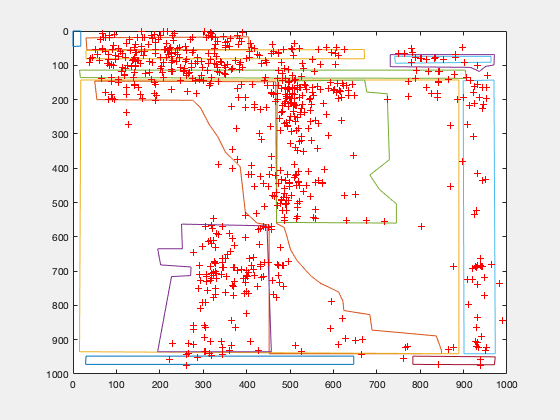
\includegraphics[scale=0.8]{CARICAMENTI_TESI/Caricamento_7_8_dicembre_2020/7_caricamento_8_dicembre_2020/analisi_semantica_immagini/economist_daily_chart_4/POLY_AND_POINTS_economist_daily_chart_4}
%\caption{...}\label{fig: POLY_AND_POINTS_economist_daily_chart_4}
%\end{figure}

\section{Testo} 


Alla luce di quanto abbiamo visto in precedenza, ovvero il fatto che Matzen suddivida l'analisi in due parti per poi assemblare insieme i risultati, e in base alle ricerche secondo le quali il testo è ciò che maggiormente attira l'attenzione dell'occhio umano, potrebbero sorgere spontanee alcune domande: 
\\\\
-"Non è che Matzen prevale sugli altri due algoritmi (Itti ed Itti Modificato) solamente perchè è presente del testo?"

-"Se dall'immagine tagliamo il titolo oppure altre parti di testo, come performa a livello di risultati sulle metriche rispetto agli altri due?"

-"Dopo aver tagliato l'immagine escludendo parte del testo, come performa invece confrontandolo con i punti veri di fissazione degli osservatori?"
\\\\
L'obiettivo di questa parte è proprio quello di rispondere a queste domande per magari cercare di scoprire qualcosa di nuovo. 

A questo scopo abbiamo preso in osservazione 11 immagini di \textit{MASSVIS} e abbiamo effettuato dei tagli andando ad escludere alcune delle parti di testo. Alcune le abbiamo tagliate anche più volte lasciando fuori magari prima solo il titolo, poi altre parti come ad esempio la legenda. Controllare la sezione 4.3 di questo documento relativa al materiale allegato per vedere meglio come è organizzato tutto il materiale che abbiamo elaborato nel corso di questi mesi per questo lavoro di tesi.

Dopo aver effettuato i tagli abbiamo ripetuto tramite codice Matlab le stesse analisi che abbiamo già raccontato nelle parti precedenti di questo documento: 
\begin{itemize}
\item abbiamo prodotto la mappa di calore relativa ai punti di fissazione degli osservatori (quelli che non rientrano più nella nuova immagine tagliata non sono stati presi in considerazione);
\item abbiamo eseguito l'algoritmo di Matzen che genera la sua mappa di calore di previsione dell'attenzione dell'occhio umano;
\item abbiamo successivamente calcolato le metriche confrontando la mappa prodotta da itti, Itti modificato e Matzen con la vera mappa di calore dei punti di fissazione degli osservatori.
\end{itemize}
\begin{figure}[!htb]\centering
\begin{subfigure}
\centering
\includegraphics[scale=0.31]{CARICAMENTI_TESI/Caricamento_3_2_novembre_2020/3_caricamento_2_novembre_2020/crop_images/economist_daily_chart_4/CROP_1/EyeTracking_economist_daily_chart_4}
\end{subfigure}
\begin{subfigure}
\centering
\includegraphics[scale=0.3]{CARICAMENTI_TESI/Caricamento_3_2_novembre_2020/3_caricamento_2_novembre_2020/crop_images/economist_daily_chart_4/CROP_1/Final_economist_daily_chart_4}
\end{subfigure}
\begin{subfigure}
\centering
\includegraphics[scale=0.31]{CARICAMENTI_TESI/Caricamento_3_2_novembre_2020/3_caricamento_2_novembre_2020/crop_images/economist_daily_chart_5/CROP_1/EyeTracking_economist_daily_chart_5}
\end{subfigure}
\begin{subfigure}
\centering
\includegraphics[scale=0.3]{CARICAMENTI_TESI/Caricamento_3_2_novembre_2020/3_caricamento_2_novembre_2020/crop_images/economist_daily_chart_5/CROP_1/Final_economist_daily_chart_5}
\end{subfigure}
\caption{Analisi sul testo}\label{fig: Final_economist_daily_chart_4_CROP}
\end{figure}
In figura \ref{fig: Final_economist_daily_chart_4_CROP} sono contenuti due esempi di quello che abbiamo svolto su due delle immagini di \textit{MASSVIS}: \textit{economist\_daily\_chart\_4} e \textit{economist\_daily\_chart\_5}. A sinistra è contenuta l'immagine ritagliata con sovrapposta la mappa di calore dei punti di fissazione, mentre a destra è contenuta la mappa di calore prodotta da Matzen. In questi due casi particolari mostrati, nel ritaglio che abbiamo adoperato siamo andati ad escludere rispetto alle immagini originali il titolo. 

Possiamo incominciare a notare come rispetto ai risultati grafici in figura \ref{fig: EyeTracking_economist_daily_chart_4} Matzen inizi ad andare un pò in confusione nel rappresentare la corretta porzione dell'immagine sulla quale con buona probabilità l'attenzione dell'occhio si andrà a concentrare. In particolare nell'immagine in alto possiamo notare che appena il titolo non è più presente, Matzen va a scegliere in maniera quasi uniforme tutta la restante porzione di testo (cosa che logicamente non è corretta perchè viene ricoperta una porzione troppo estesa con la saliency). Similmente, ma in maniera meno accentuata, questo accade anche nell'immagine sottostante in cui però comunque Matzen continua ad indicare in maniera corretta la porzione più saliente in base a ciò che produce.

Quello che ora bisogna capire è se comunque l'algoritmo di Matzen, nonostante questo difetto di concentrarsi su tutto il testo a disposizione in maniera quasi uniforme una volta che il titolo sparisce, sia ancora l'algoritmo più efficiente rispetto a quello di Itti e rispetto a quello di Itti modificato.
A tal proposito nella tabella \ref{t:2} sono presenti tre sezioni in cui vengono mostrati i risultati delle metriche confrontando due algoritmi alla volta come già fatto nella sezione precedente con la tabella \ref{t:1}.



%\begin{figure}[!htb]\centering
%\includegraphics[scale=0.7]{CARICAMENTI_TESI/Caricamento_3_2_novembre_2020/3_caricamento_2_novembre_2020/crop_images/economist_daily_chart_4/CROP_1/EyeTracking_economist_daily_chart_4}
%\caption{...}\label{fig: EyeTracking_economist_daily_chart_4}
%\end{figure}

\begin{table}[htp]
\small              
\centering                      
\begin{tabular} %{lllllll}   
%{c}               
{l c c c c c c c c}                  % parametri di incolonnamento: r (a destra), c (al centro), l (a sinistra),% p (per definire la larghezza della colonna)
\hline\hline
& AUC-Borji &  AUC-Judd &  AUC-S. &  CC &  EMD &  KL &  NSS &  SIM  \\  
\hline
%\hspace*{1.3em}
ITTI OR & 20\% & 25\%  & 50\% & 45\% & 40\%  & 80\%  & 25\%  &  25\% \\
ITTI MOD & 75\% & 75\% & 50\% & 50\% & 60\% & 20\% & 75\% & 75\%\\
PAREGGIO & 5\% & 0\%  & 0\% & 5\% & 0\% & 0\% & 0\% & 0\%\\
\hline \hline
& AUC-Borji &  AUC-Judd &  AUC-S. &  CC &  EMD &  KL &  NSS &  SIM  \\  
\hline
%\hspace*{1.3em}
MATZEN & 85\% & 85\%  & 80\% & 80\% & 25\%  & 10\%  & 95\% & 70\% \\
ITTI OR & 15\% & 15\%  &   20\%  & 20\% & 75\%  & 90\%  & 5\%  &  30\%\\
PAREGGIO & 0\% & 0\%  &  0\%  & 0\% & 0\%  & 0\%  & 0\% &  0\%\\
\hline \hline
& AUC-Borji &  AUC-Judd &  AUC-S. &  CC &  EMD &  KL &  NSS &  SIM  \\  
\hline
%\hspace*{1.3em}
MATZEN & 85\% & 85\%  & 90\% & 80\% & 20\%  & 10\%  & 95\%  &  65\% \\
ITTI MOD & 15\% & 10\%  &   10\%  & 15\% & 75\%  & 85\%  & 0\%  &  30\%\\
PAREGGIO & 0\% & 5\% & 0\% & 5\% & 5\%  & 5\%  & 5\%  &  5\%\\
\hline \hline
\end{tabular}
\caption[Risultati metriche analisi sul testo]{Risultati metriche analisi sul testo} \label{t:2}  
%[Short description for the content list.]{Complete descreption: caption of the table.}
\end{table}

Quello che possiamo notare analizzando questi risultati sulle percentuali di vittorie è che: tagliando parte del testo Matzen peggiora le sue prestazioni a livello di regioni dell'immagine in cui si prevede che l'attenzione si concentrerà, ma rimane comunque l'algoritmo di previsione migliore (rispetto ad Itti ed Itti modificato) a livello numerico  sulle metriche.
%\begin{table}[htp]              
%\centering                      
%\begin{tabular} %{lllllll}   
%%{c}               
%{l c c c c c c c c}                  % parametri di incolonnamento: r (a destra), c (al centro), l (a sinistra), % p (per definire la larghezza della colonna)
%\hline\hline
%& AUC-Borji &  AUC-Judd &  AUC-Shuffled &  CC &  EMD &  KL &  NSS &  SIM  \\  
%\hline
%%\hspace*{1.3em}
%MATZEN & 85\% & 85\%  & 80\% & 80\% & 25\%  & 10\%  & 95\% & 70\% \\
%ITTI OR & 15\% & 15\%  &   20\%  & 20\% & 75\%  & 90\%  & 5\%  &  30\%\\
%PAREGGIO & 0\% & 0\%  &  0\%  & 0\% & 0\%  & 0\%  & 0\% &  0\%\\
%\hline \hline
%\end{tabular}
%\caption[Descrizione breve: compare nell'elenco tabelle]{...(scrivi)...} \label{t:1}  
%%[Short description for the content list.]{Complete descreption: caption of the table.}
%\end{table}
%
%\begin{table}[H]              
%\centering                      
%\begin{tabular} %{lllllll}   
%%{c}               
%{l c c c c c c c c}                  % parametri di incolonnamento: r (a destra), c (al centro), l (a sinistra),	% p (per definire la larghezza della colonna)
%\hline\hline
%& AUC-Borji &  AUC-Judd &  AUC-Shuffled &  CC &  EMD &  KL &  NSS &  SIM  \\  
%\hline
%%\hspace*{1.3em}
%MATZEN & 85\% & 85\%  & 90\% & 80\% & 20\%  & 10\%  & 95\%  &  65\% \\
%ITTI MOD & 15\% & 15\%  &   10\%  & 20\% & 80\%  & 90\%  & 5\%  &  35\%\\
%PAREGGIO & 0\% & 5\% & 0\% & 5\% & 5\%  & 5\%  & 5\%  &  5\%\\
%\hline \hline
%\end{tabular}
%\caption[Descrizione breve: compare nell'elenco tabelle]{...(scrivi)...} \label{t:1}  
%%[Short description for the content list.]{Complete descreption: caption of the table.}
%\end{table}



\chapter{Esperimento con l'eyetracker}

\section{Raccolta dei dati e dataset}
Dato che le analisi svolte nel capitolo precedente erano legate ad un dataset già presente online e non controllato da noi, abbiamo pensato di crearne uno nuovo da zero, con le caratteristiche che volevamo e che abbiamo deciso noi, con lo scopo di  poter effettuare un nostro esperimento in maniera autonoma.

\begin{figure}[!htb]\centering
\begin{subfigure}
\centering
\includegraphics[scale=0.2]{IMMAGINI_ESPERIMENTO_ORIGINALI/graph0}
%\caption{...(prova)...}
\end{subfigure}
\begin{subfigure}
\centering
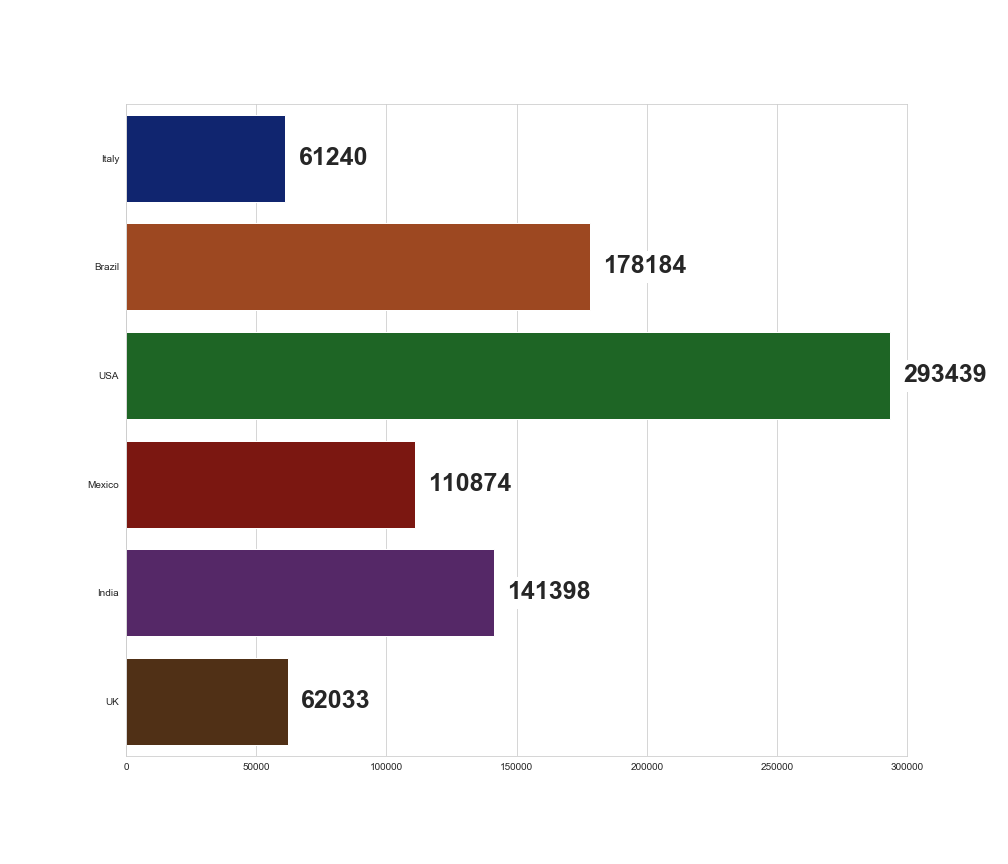
\includegraphics[scale=0.2]{IMMAGINI_ESPERIMENTO_ORIGINALI/graph11}
\end{subfigure}
\begin{subfigure}
\centering
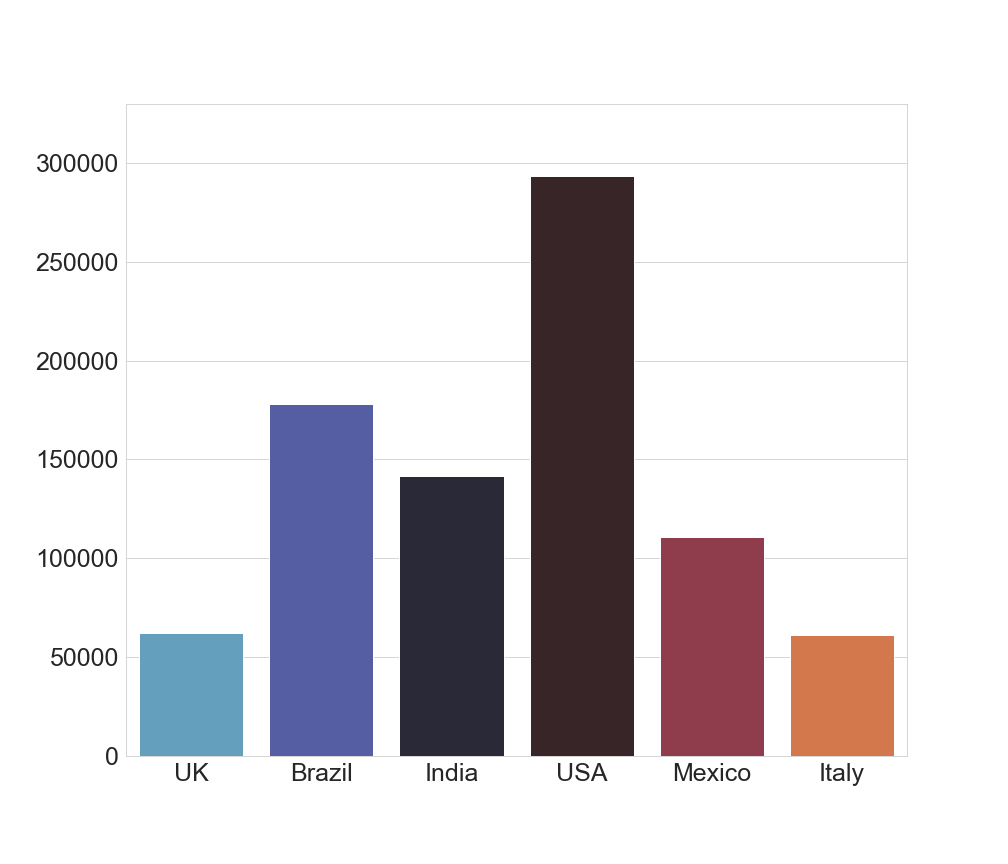
\includegraphics[scale=0.2]{IMMAGINI_ESPERIMENTO_ORIGINALI/graph6}
\end{subfigure}
\begin{subfigure}
\centering
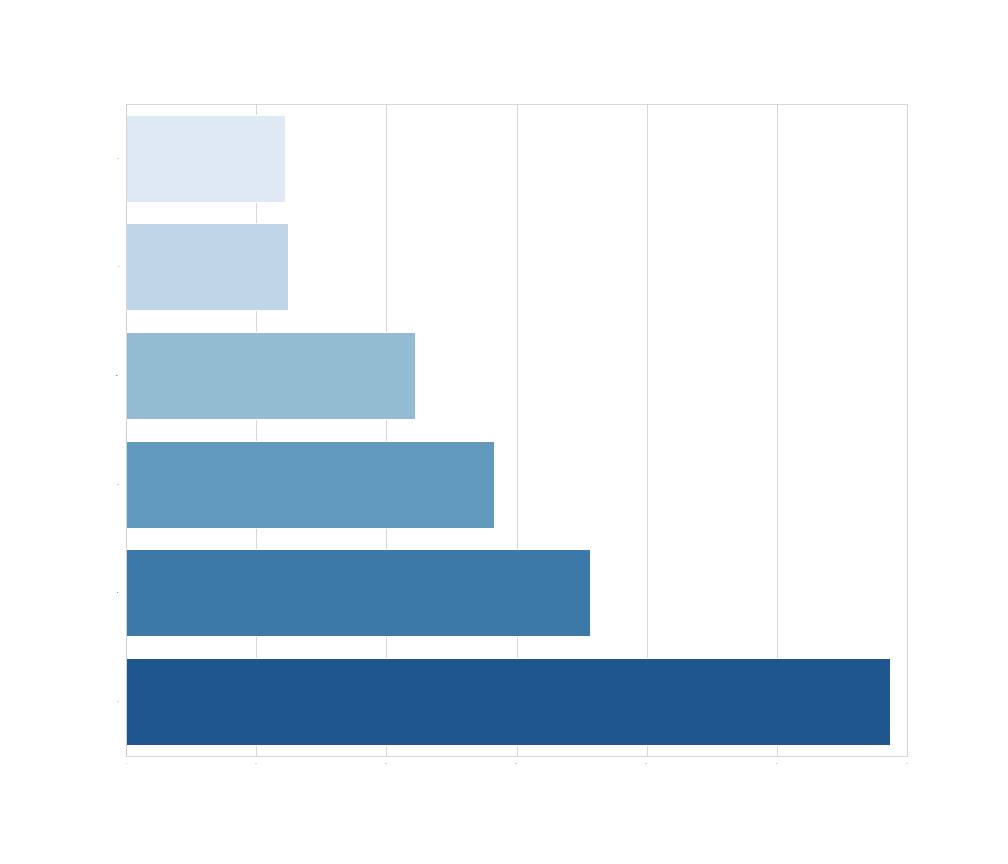
\includegraphics[scale=0.2]{IMMAGINI_ESPERIMENTO_ORIGINALI/graph17}
\end{subfigure}
\begin{subfigure}
\centering
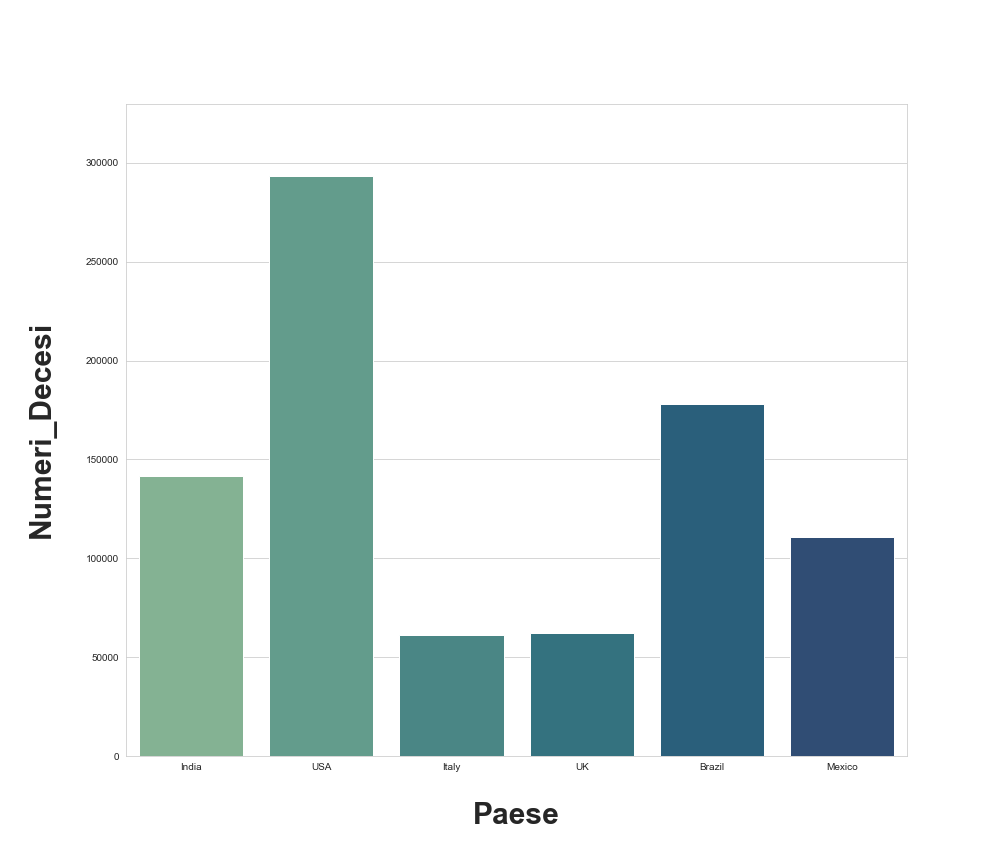
\includegraphics[scale=0.2]{IMMAGINI_ESPERIMENTO_ORIGINALI/graph5}
\end{subfigure}
\caption{Dataset esperimento eye-tracker}\label{fig: graphs}
\end{figure}

A tal proposito abbiamo creato 30 immagini tutte relative ad una caratteristica di base: si tratta di grafici a barre, cioè di istogrammi, relativi all'epidemia di \textit{COVID-19} e ai dati dei decessi in alcuni paesi del mondo. Partendo da questo elemento di base abbiamo poi costruito le immagini effettuando alcune piccole varianti tra una e l'altra che sono elencate qui di seguito:
\begin{itemize}
\item \textit{barre orizzontali/verticali}: alcune immagini hanno le barre disposte orizzontalmente e alcune verticalmente;
\item \textit{titolo sì/no}: alcune immagini hanno il titolo in alto con il relativo sottotitolo e altre no;
\item \textit{titolo assi sì/no}: alcune immagini hanno il titolo sui due assi e altre no;
\item \textit{etichette barre sì/no}: alcune immagini hanno i numeri associati alla grandezza di ogni singola barra e altre no;
\item \textit{etichette assi sì/no}: alcune immagini contengono il valore numerico o l'etichetta di testo sugli assi e altre no;
\item \textit{etichette assi grandi/piccole}: in alcune tra le immagini che contengono l'etichetta sugli assi è stato utilizzato un carattere più piccolo e altre in altre un pò più grande;
\item \textit{colori accesi/tenui}: alcune immagini hanno le barre con colori accesi e altre invece le hanno con colori tenui;
\item \textit{colori diversi/scala unico colore}: alcune immagini contengono le barre che hanno colori diversi e invece in altre è presente la scala di un unico colore.
\end{itemize}


\begin{figure}[H]\centering
\includegraphics[scale=0.6]{SCREEN_TESI/Caratteristiche_immagini_dataset}
\caption{Distribuzione caratteristiche immagini dataset esperimento eye tracker}\label{fig: figura_distribuzione_caratteristiche}
\end{figure}

In figura \ref{fig: graphs} sono contenute 5 delle 30 immagini totali che rappresentano un pò i prototipi di tutte le caratteristiche che ho elencato in precedenza. In  \ref{fig: figura_distribuzione_caratteristiche} abbiamo invece un riassunto in formato di tabella che descrive un pò come sono distribuite le caratteristiche tra le varie immagini del nostro dataset. Ricordo che nella sezione 4.3 viene descritto come è organizzato tutto il materiale elaborato da noi durante questi mesi di lavoro alla tesi. Sarà disponibile insieme a questo documento e oltre a tutte le informazioni che abbiamo prodotto su \textit{MASSVIS} e discusse nel capitolo precedente conterrà anche le informazioni riguardanti il nostro esperimento.

La tabella \ref{t:3} descrive come è distribuito il campione di osservatori al quale è stato sottoposto l'esperimento. In totale gli osservatori sono 62 e le loro caratteristiche sono appunto descritte in tabella. 



%\begin{figure}[!htb]\centering
%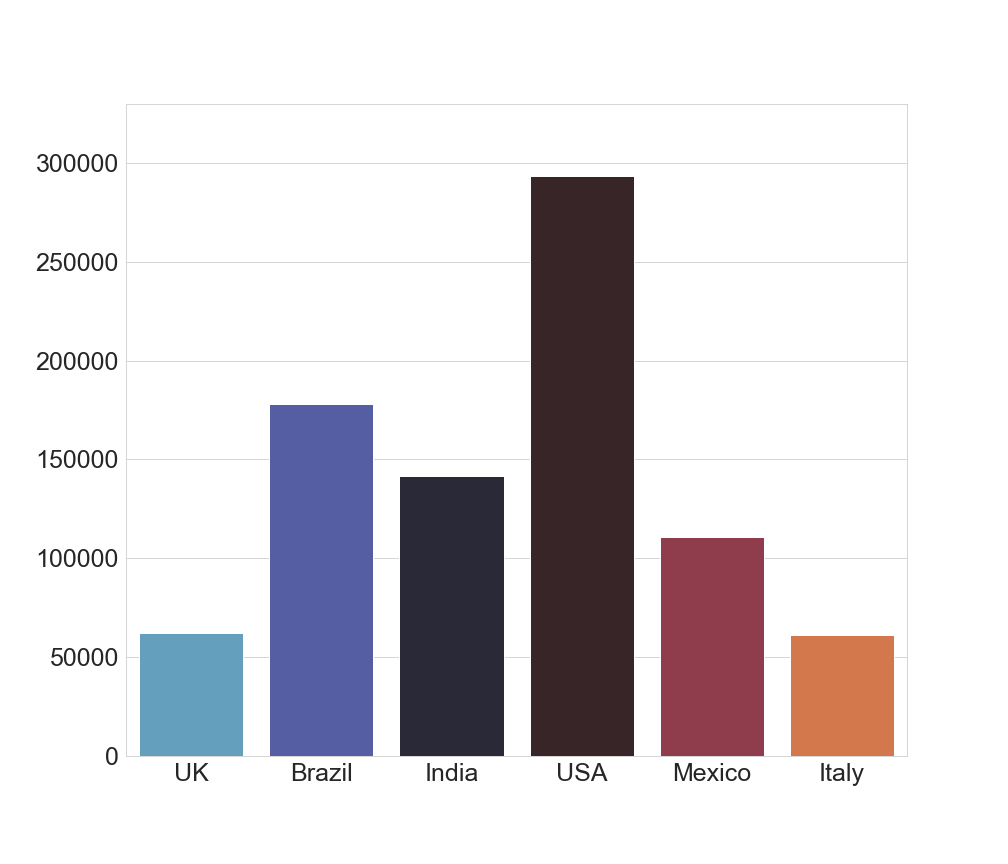
\includegraphics[scale=0.45]{IMMAGINI_ESPERIMENTO_ORIGINALI/graph6}
%\caption{...}\label{fig: graph6}
%\end{figure}


%\begin{figure}[!htb]\centering
%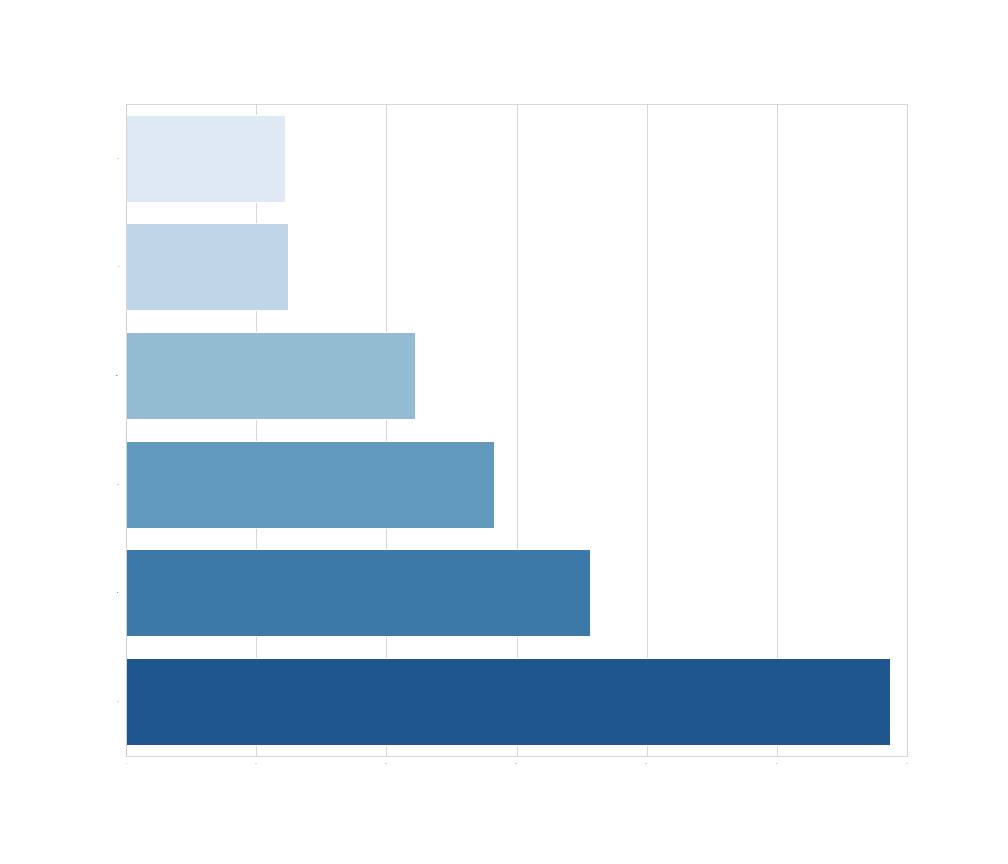
\includegraphics[scale=0.45]{IMMAGINI_ESPERIMENTO_ORIGINALI/graph17}
%\caption{...}\label{fig: graph17}
%\end{figure}

%\begin{figure}[!htb]\centering
%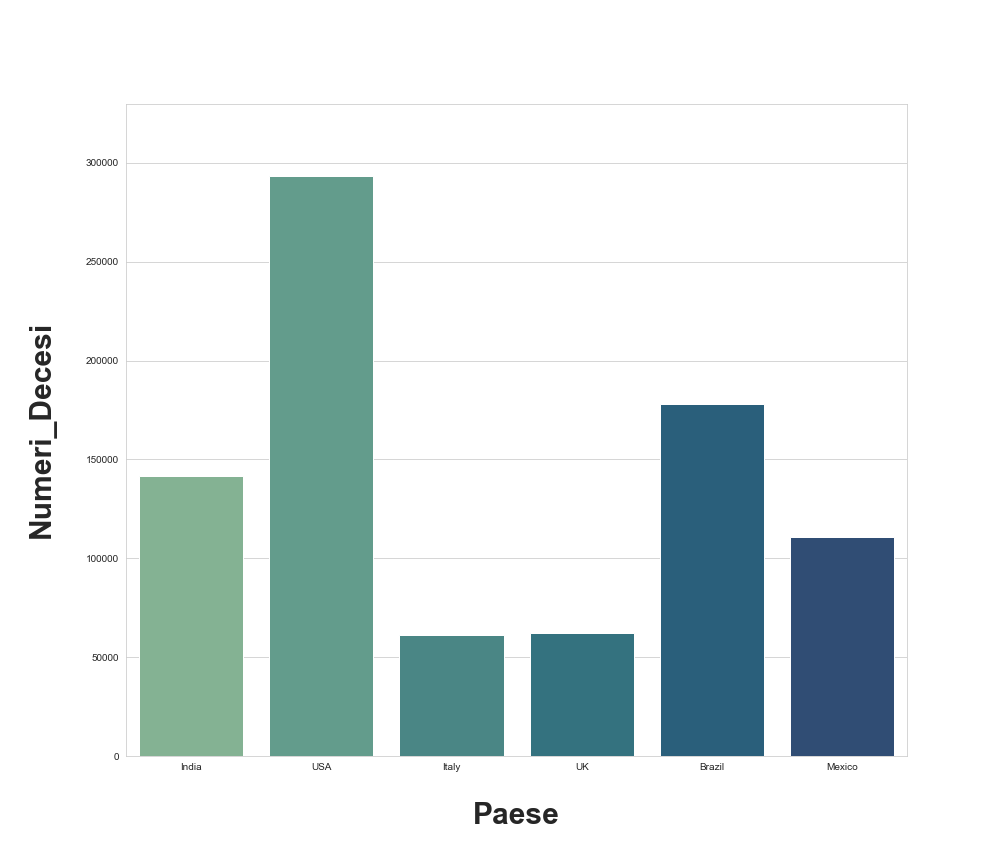
\includegraphics[scale=0.45]{IMMAGINI_ESPERIMENTO_ORIGINALI/graph5}
%\caption{...}\label{fig: graph5}
%\end{figure}


\begin{table}[htb]              
\centering                      
\begin{tabular} %{lllllll}   
%{c}               
{l c c c c c c c c}                  % parametri di incolonnamento: r (a destra), c (al centro), l (a sinistra),% p (per definire la larghezza della colonna)
\hline\hline
& 14/18 &  24/30 &  45/50  \\  
\hline
\hspace*{1.3em}
ETA' & 51 & 3 & 8 \\
\hline\hline

\hline\hline
\hspace{1.3em}
& F &  M &   \\  
\hline
\hspace*{1.3em}
SESSO & 5 & 57 & \\
\hline \hline
\end{tabular}
\caption[Campione esperimento eye tracker]{Campione esperimento eye tracker} \label{t:3}  
%[Short description for the content list.]{Complete descreption: caption of the table.}
\end{table}

Ci rendiamo conto che il campione non è distribuito in maniera bilanciata (sia per quanto riguarda l'età e sia per quanto riguarda il sesso), però visto il periodo di emergenza sanitaria durante questi mesi in cui abbiamo portato avanti il lavoro di tesi non è stato possibile raccogliere in tempi brevi un insieme di osservatori con caratteristiche più varie e ci riteniamo fortunati già solo di poter aver effettuato l'esperimento.

Il Politecnico di Torino ci ha permesso di attrezzarci adeguatamente e siamo potuti entrare in possesso di un eye tracker con cui effettuare le varie prove: in particolare è stato adoperato il modello \href{https://www.tobiipro.com/product-listing/nano/}{\texit{Tobii Pro Nano}}, mentre l'esperimento è stato svolto usando l'applicazione \textit{Open Sesame}.

L'esperimento si è svolto come segue: 
\begin{itemize}
\item inizialmente ogni osservatore è stato posizionato davanti al computer al quale è stato collegato l'eye tracker;
\item in seguito è stata eseguita la calibrazione dell'eye tracker sull'osservatore;
\item dopodichè è iniziato il vero e proprio esperimento in cui ogni osservatore ha visualizzato ciascuna delle 30 immagini del dataset per 5 secondi in ordine casuale.
\end{itemize}

Sottlineiamo che tra un'immagine e la successiva è stata inserita la pressione di un tasto della tastiera per permettere all'osservatore di riposizionarsi con lo sguardo nella parte centrale dello schermo. Questo ultimo passaggio è stato svolto con lo scopo di evitare che da un'immagine a quella successiva ci si portasse dietro un errore dovuto alla transizione tra una e l'altra senza la presenza di uno stacco di nessun tipo tra le due immagini.

\newpage
\section{Analisi sui dati raccolti}
\begin{figure}[!htb]\centering
\begin{subfigure}
\centering
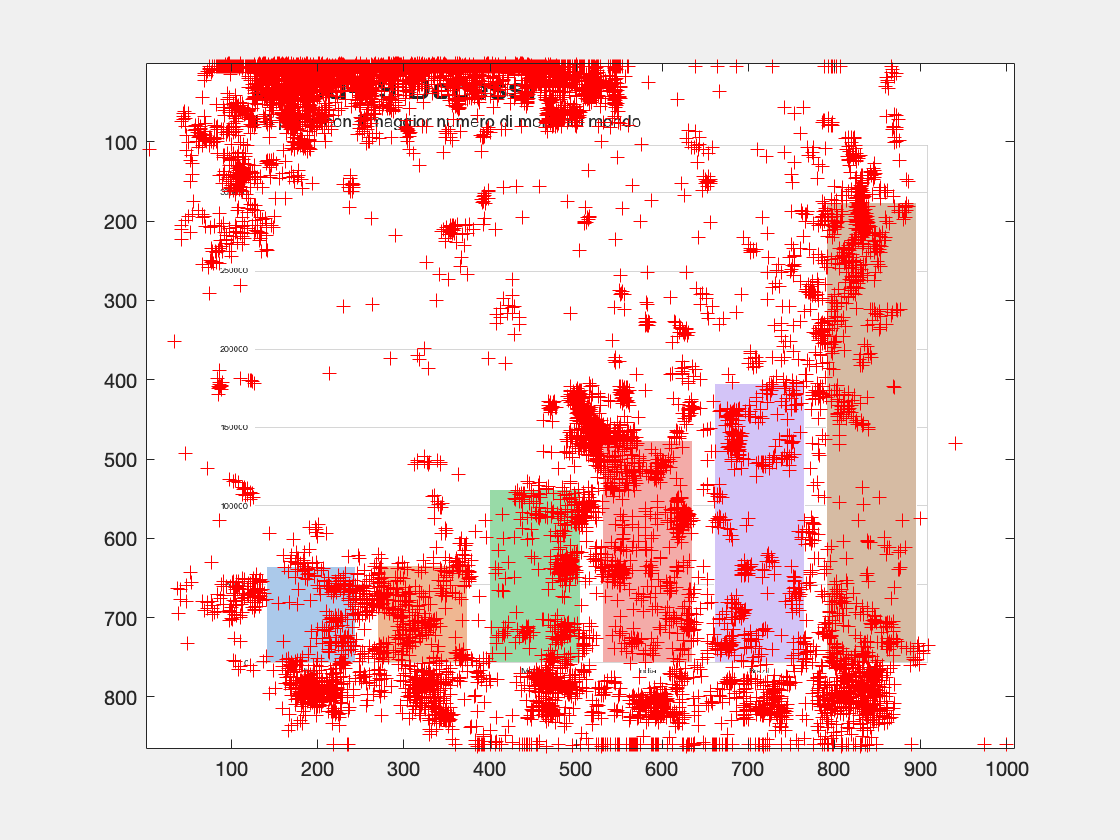
\includegraphics[scale=0.22]{CARICAMENTI_TESI/Caricamento_12_19_gennaio_2021/IMMAGINI_ESPERIMENTO_19_gennaio_2021/im0/IMAGE_FIXATIONS_62_graph0}
\end{subfigure}
\begin{subfigure}
\centering
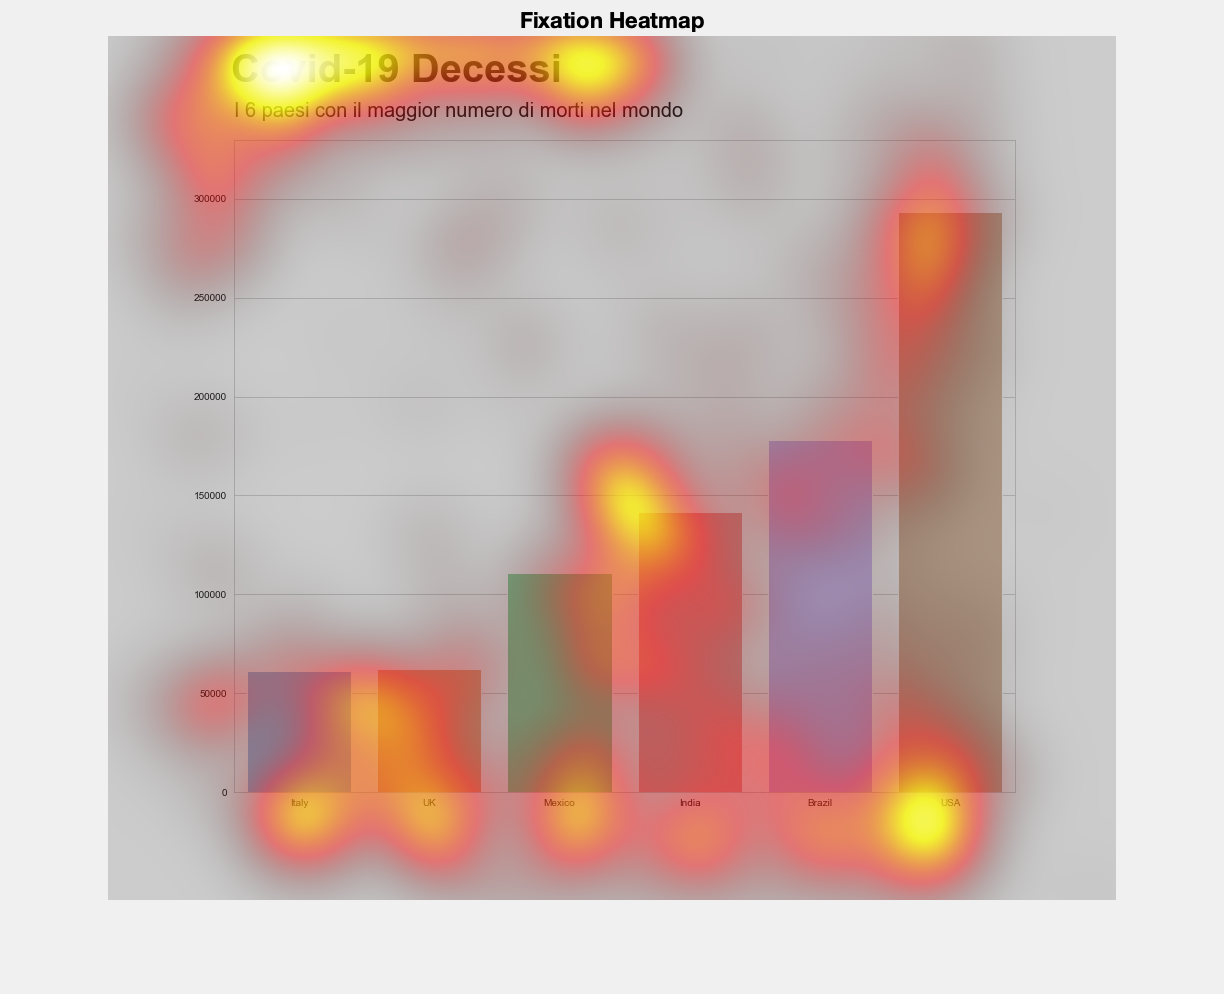
\includegraphics[scale=0.2]{CARICAMENTI_TESI/Caricamento_12_19_gennaio_2021/IMMAGINI_ESPERIMENTO_19_gennaio_2021/im0/IMAGE_HEAT_MAP_62_graph0}
\end{subfigure}
\begin{subfigure}
\centering
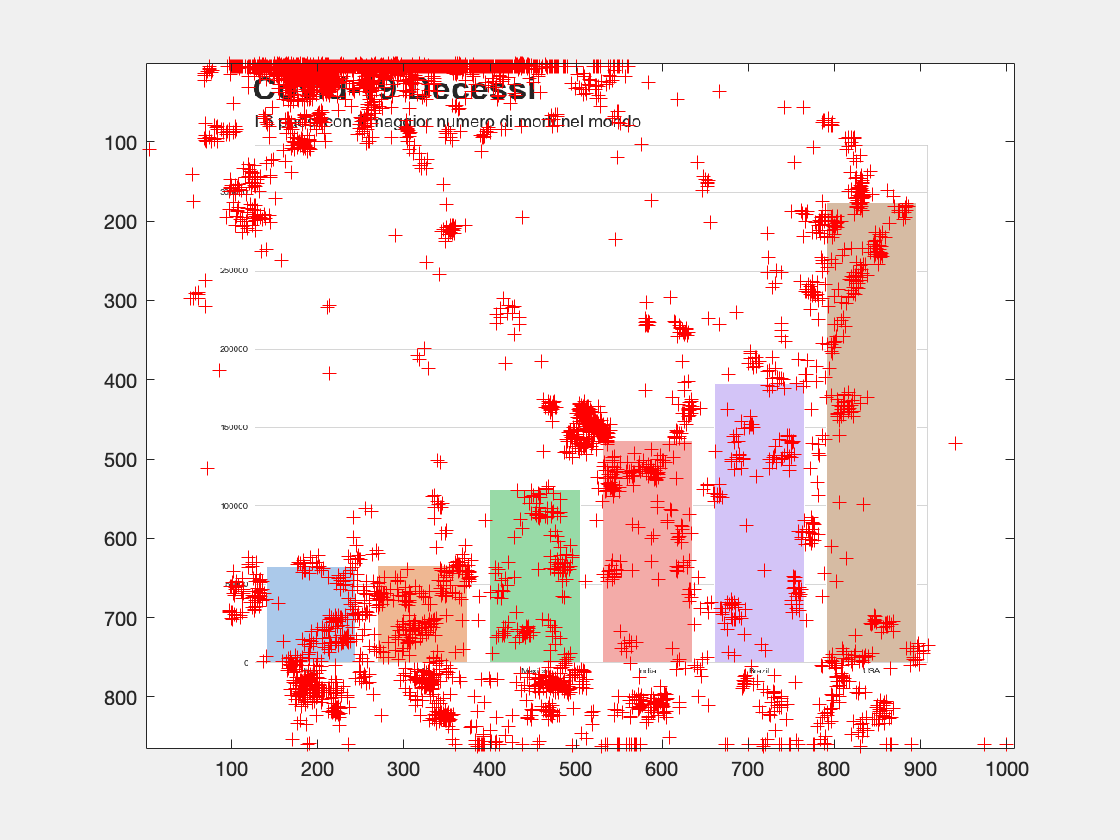
\includegraphics[scale=0.22]{CARICAMENTI_TESI/Caricamento_12_19_gennaio_2021/IMMAGINI_ESPERIMENTO_19_gennaio_2021/im0/FIRST_IMAGE_FIXATIONS_62_graph0}
\end{subfigure}
\begin{subfigure}
\centering
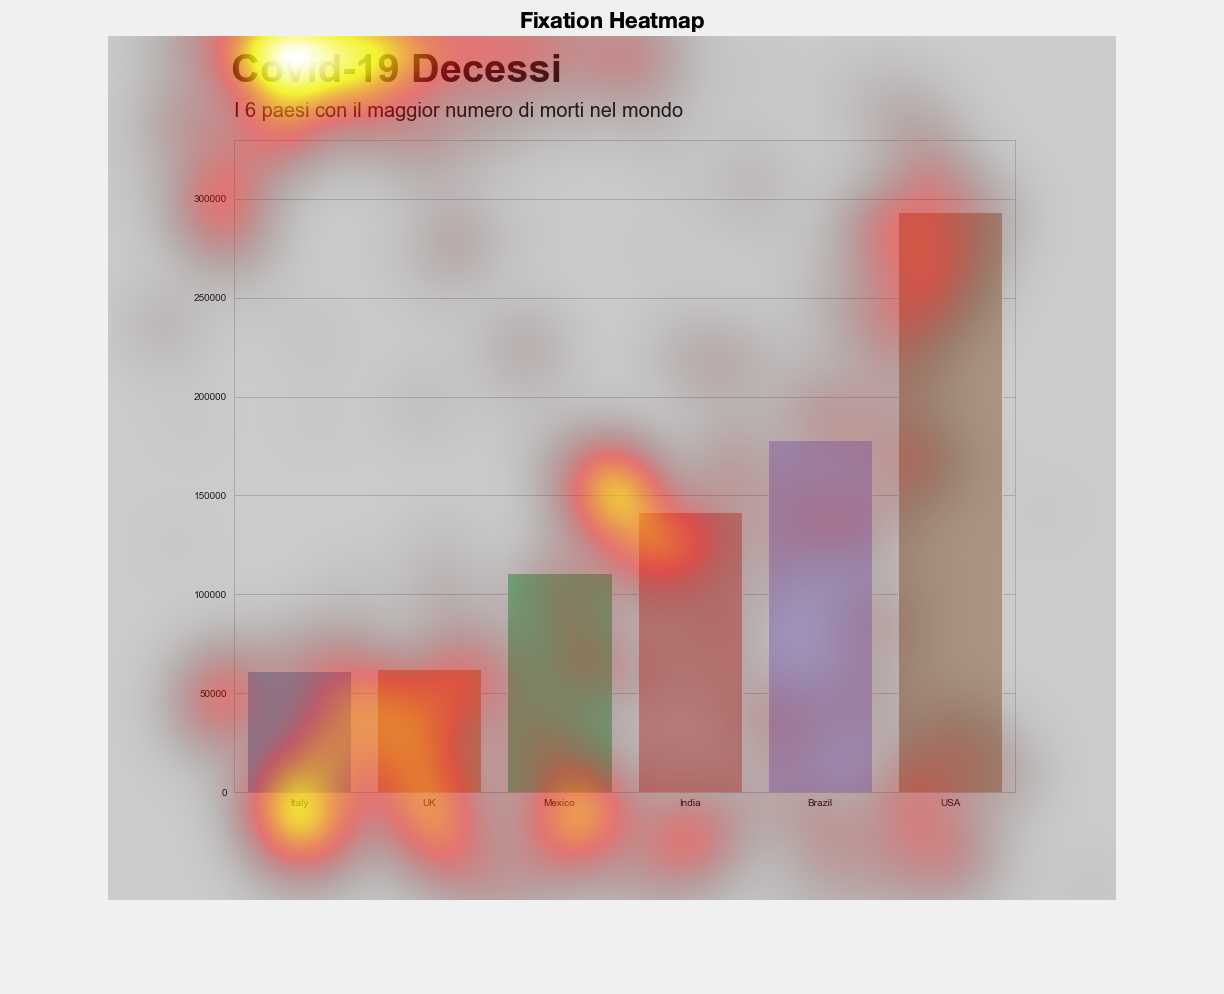
\includegraphics[scale=0.2]{CARICAMENTI_TESI/Caricamento_12_19_gennaio_2021/IMMAGINI_ESPERIMENTO_19_gennaio_2021/im0/FIRST_IMAGE_HEAT_MAP_62_graph0}
\end{subfigure}
\begin{subfigure}
\centering
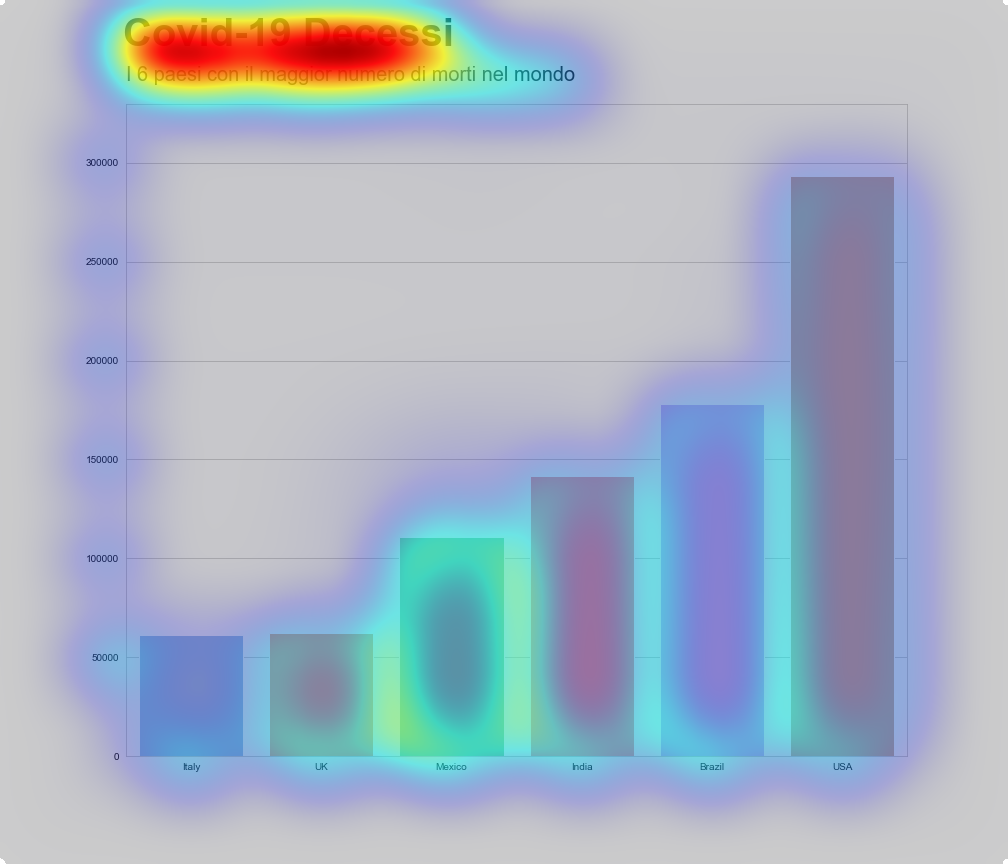
\includegraphics[scale=0.2]{CARICAMENTI_TESI/Caricamento_12_19_gennaio_2021/IMMAGINI_ESPERIMENTO_19_gennaio_2021/im0/mySalience_graph0}
\end{subfigure}
\caption{Punti di fissazione - Mappa di calore (globale e pre-attentive)}\label{fig: IMAGE_FIXATIONS_62_graph0}
\end{figure}

Per ogni osservatore, cioè ogni volta in cui l'esperimento viene ripetuto, l'eye tracker produce in uscita un file di testo contenente tutte le informazioni necessarie per le analisi. I dati sono poi stati ripuliti di informazioni accessorie e non utili. 
Per quanto riguarda l'esperimento eseguito, abbiamo per ogni immagine e per ogni osservatore i seguenti dati:
\begin{itemize}
\item  un file di testo contenente tutti i punti di osservazione per quell'immagine raccolti ogni 15 ms;
\item un file excel che è il contenuto del file di testo convertito in formato tabellare per essere agevolmente importato in Matlab.
\end{itemize}

Con questi dati ci siamo spostati in Matlab ad eseguire i medesimi passaggi che abbiamo svolto con \textit{MASSVIS} e che sono descritti nel capitolo precedente. In particolare in questa sezione quello che viene mostrato è: 

\begin{itemize}
\item in figura \ref{fig: IMAGE_FIXATIONS_62_graph0} l'immagine originale \textit{graph0} con sovrapposti i punti di fissazione  con la relativa mappa di calore a fianco associata, le stesse due figure con solo i punti presi nei primi 2,5 s (per osservare la presenza o meno di qualche differenza nella fase preattentive) e la mappa di salienza prodotta da Matzen;
\item in figura \ref{fig: IMAGE_FIXATIONS_62_graph5} le stesse informazioni di sopra, ma relative all'immagine \textit{graph5};
\item in figura \ref{fig: IMAGE_FIXATIONS_62_graph11} le informazioni relative rispettivamente alle immagini \textit{graph11} e \textit{graph6} in cui non si è analizzata la fase preattentive semplicemente per non caricare di ulteriori immagini il documento (tutto il materiale completo è comunque disponibile e descritto nella sezione 4.3).
\end{itemize}

Le osservazioni e i commenti a queste figure sono lasciati nella prossima sezione in cui vengono analizzati i risultati grafici delle analisi che sono appena state raccontate e anche i dati numerici di prestazione con le metriche.


\begin{figure}[!htb]\centering
\begin{subfigure}
\centering
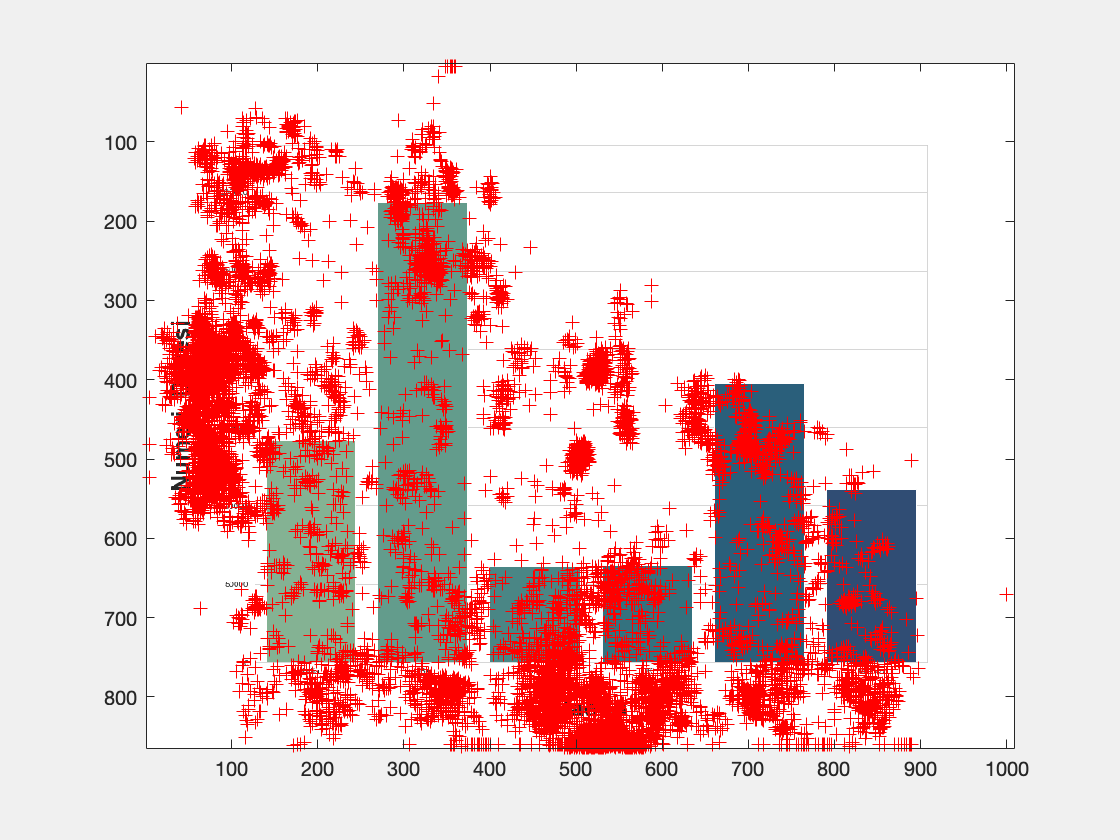
\includegraphics[scale=0.22]{CARICAMENTI_TESI/Caricamento_12_19_gennaio_2021/IMMAGINI_ESPERIMENTO_19_gennaio_2021/im5/IMAGE_FIXATIONS_62_graph5}
\end{subfigure}
\begin{subfigure}
\centering
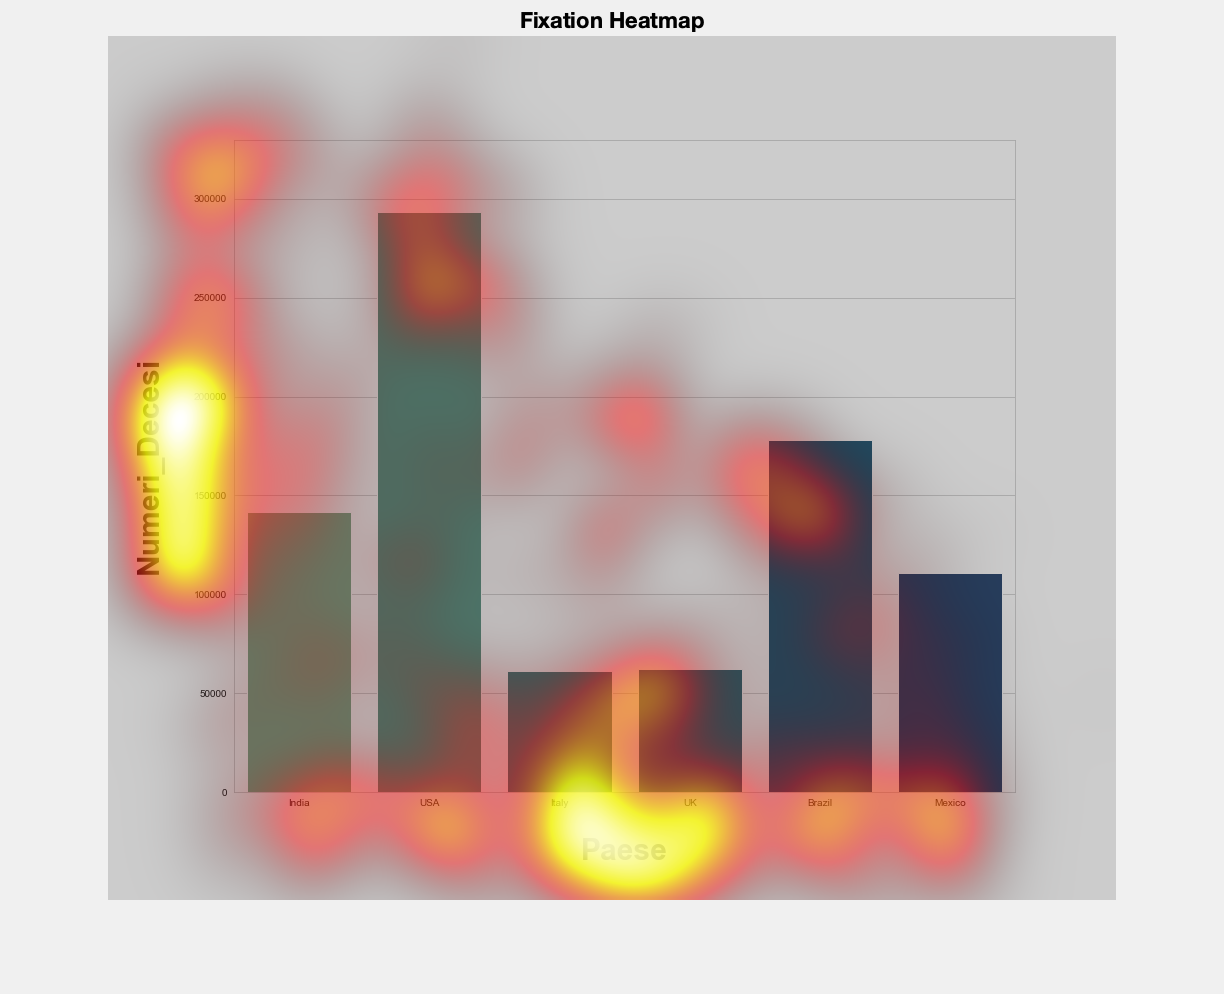
\includegraphics[scale=0.2]{CARICAMENTI_TESI/Caricamento_12_19_gennaio_2021/IMMAGINI_ESPERIMENTO_19_gennaio_2021/im5/IMAGE_HEAT_MAP_62_graph5}
\end{subfigure}
\begin{subfigure}
\centering
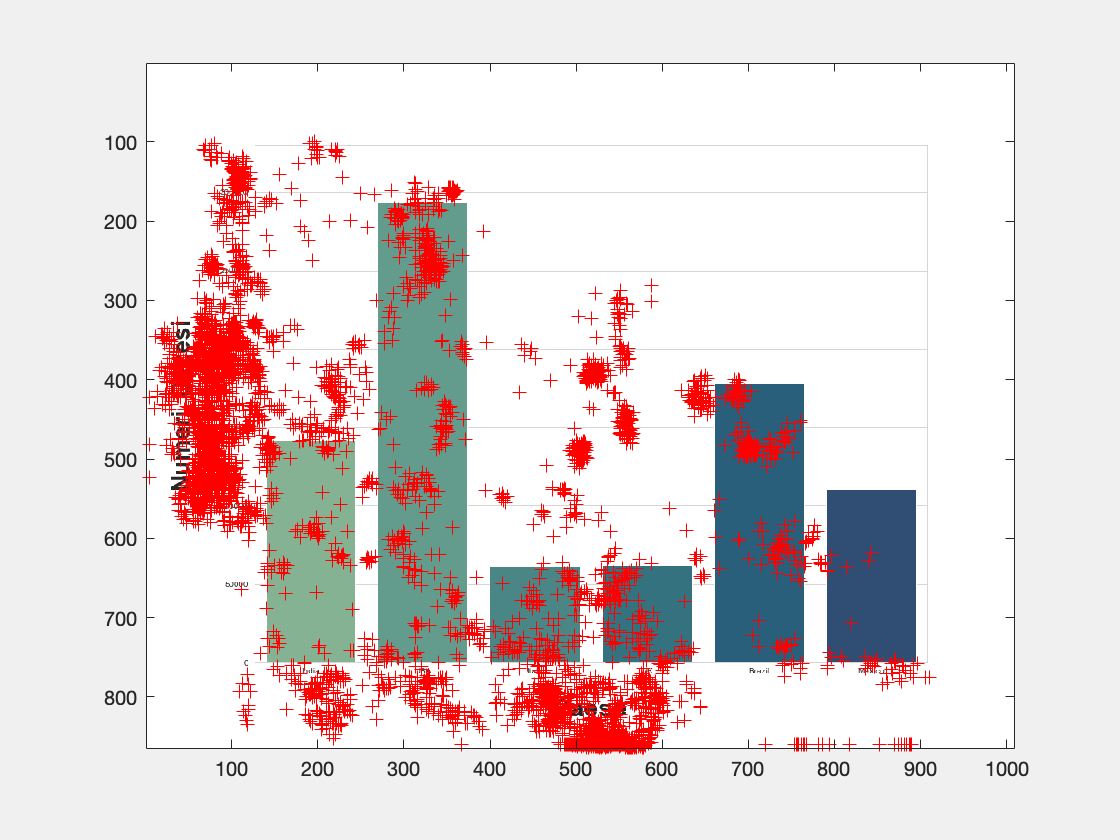
\includegraphics[scale=0.22]{CARICAMENTI_TESI/Caricamento_12_19_gennaio_2021/IMMAGINI_ESPERIMENTO_19_gennaio_2021/im5/FIRST_IMAGE_FIXATIONS_62_graph5}
\end{subfigure}
\begin{subfigure}
\centering
\includegraphics[scale=0.2]{CARICAMENTI_TESI/Caricamento_12_19_gennaio_2021/IMMAGINI_ESPERIMENTO_19_gennaio_2021/im5/FIRST_IMAGE_HEAT_MAP_62_graph5}
\end{subfigure}
\begin{subfigure}
\centering
\includegraphics[scale=0.2]{CARICAMENTI_TESI/Caricamento_12_19_gennaio_2021/IMMAGINI_ESPERIMENTO_19_gennaio_2021/im5/mySalience_graph5}
\end{subfigure}
\caption{Punti di fissazione - Mappa di calore (globale e pre-attentive)}\label{fig: IMAGE_FIXATIONS_62_graph5}
\end{figure}

\begin{figure}[!htb]\centering
\begin{subfigure}
\centering
\includegraphics[scale=0.22]{CARICAMENTI_TESI/Caricamento_12_19_gennaio_2021/IMMAGINI_ESPERIMENTO_19_gennaio_2021/im11/IMAGE_FIXATIONS_62_graph11}
\end{subfigure}
\begin{subfigure}
\centering
\includegraphics[scale=0.2]{CARICAMENTI_TESI/Caricamento_12_19_gennaio_2021/IMMAGINI_ESPERIMENTO_19_gennaio_2021/im11/IMAGE_HEAT_MAP_62_graph11}
\end{subfigure}
\begin{subfigure}
\centering
\includegraphics[scale=0.22]{CARICAMENTI_TESI/Caricamento_12_19_gennaio_2021/IMMAGINI_ESPERIMENTO_19_gennaio_2021/im6/IMAGE_FIXATIONS_62_graph6}
\end{subfigure}
\begin{subfigure}
\centering
\includegraphics[scale=0.2]{CARICAMENTI_TESI/Caricamento_12_19_gennaio_2021/IMMAGINI_ESPERIMENTO_19_gennaio_2021/im6/IMAGE_HEAT_MAP_62_graph6}
\end{subfigure}
\begin{subfigure}
\centering
\includegraphics[scale=0.2]{CARICAMENTI_TESI/Caricamento_12_19_gennaio_2021/IMMAGINI_ESPERIMENTO_19_gennaio_2021/im11/mySalience_graph11}
\end{subfigure}
\begin{subfigure}
\centering
\includegraphics[scale=0.2]{CARICAMENTI_TESI/Caricamento_12_19_gennaio_2021/IMMAGINI_ESPERIMENTO_19_gennaio_2021/im6/mySalience_graph6}
\end{subfigure}
\caption{Punti di fissazione - Mappa di calore}\label{fig: IMAGE_FIXATIONS_62_graph11}
\end{figure}

%\begin{figure}[!htb]\centering
%\includegraphics[scale=0.45]{CARICAMENTI_TESI/Caricamento_12_19_gennaio_2021/IMMAGINI_ESPERIMENTO_19_gennaio_2021/im0/IMAGE_HEAT_MAP_62_graph0}
%\caption{...}\label{fig: IMAGE_HEAT_MAP_62_graph0}
%\end{figure}
%
%\begin{figure}[!htb]\centering
%\includegraphics[scale=0.45]{CARICAMENTI_TESI/Caricamento_12_19_gennaio_2021/IMMAGINI_ESPERIMENTO_19_gennaio_2021/im0/FIRST_IMAGE_FIXATIONS_62_graph0}
%\caption{...}\label{fig: FIRST_IMAGE_FIXATIONS_62_graph0}
%\end{figure}
%
%\begin{figure}[!htb]\centering
%\includegraphics[scale=0.45]{CARICAMENTI_TESI/Caricamento_12_19_gennaio_2021/IMMAGINI_ESPERIMENTO_19_gennaio_2021/im0/FIRST_IMAGE_HEAT_MAP_62_graph0}
%\caption{...}\label{fig: FIRST_IMAGE_HEAT_MAP_62_graph0}
%\end{figure}



\newpage 

\section{Risultati}

In questa parte andiamo a commentare sia a livello grafico che a livello numerico i risultati che sono emersi dalle analisi effettuate sui dati raccolti nel nostro esperimento.


\begin{figure}[!htb]\centering
\includegraphics[scale=0.8]{SCREEN_TESI/Saliency_immagini_dataset}
\caption{Distribuzione mappa di calore esperimento eye-tracker}\label{fig: Saliency_immagini_dataset}
\end{figure}

Dal punto di vista grafico, osservando le mappe di calore, abbiamo evidenziato alcune caratteristiche sulle quali l'attenzione si è prevalentemente concentrata che si ripetono tra le immagini. Sono mostrate in maniera riassuntiva in figura \ref{fig: Saliency_immagini_dataset} in cui per ognuna delle immagini del nostro dataset sono segnalate le caratteristiche di \textit{saliency} ad essa associate in base a quello che gli osservatori hanno visto. Le caratteristiche sono elencate e spiegate qui di seguito:
\begin{itemize}
\item \textit{barra più lunga}: significa che l'attenzione degli osservatori si è concentrata sulla barra più lunga presente nell'immagine;
\item \textit{barra colorata più accesa}: l'attenzione si è concentrata sulla barra con il colore più acceso;
\item \textit{titolo}: l'attenzione è concentrata sul titolo in alto nell'immagine (se presente);
\item \textit{titolo asse x}: l'attenzione è concentrata sul titolo dell'asse x;
\item \textit{titolo asse y}:  l'attenzione è concentrata sul titolo dell'asse y;
\item \textit{etichette asse x}: significa che l'attenzione si è concentrata sulle etichette (numeriche oppure di testo) presenti sull'asse x;
\item \textit{etichette asse y}: l'attenzione si è concentrata sulle etichette (numeriche oppure di testo) presenti sull'asse y;
\item \textit{etichette barre}: la saliency è concentrata sulle etichette numeriche delle barre;
\item \textit{scala barre}: significa che la saliency si è distribuita un pò tutte le barre (questo è comparso nelle immagini con le barre disposte in ordine crescente di lunghezza);
\item \textit{barra no più lunga no più colorata}: significa che l'attenzione si è concentrata sulla barra che non è nè la più lunga presente nell'immagine e neanche quella con il colore più acceso;
\item \textit{zona centrale}: l'attenzione si è focalizzata nel centro dell'immagine (potrebbe essere dovuto ad un ritardo dell'osservatore a muoversi con l'occhio sull'immagine a cercare informazioni).
\end{itemize}

Concentrandoci invece da un punto di vista numerico, nella tabella \ref{t:4} sono riassunti (nello stesso formato già adottato nel capitolo precedente) i risultati delle metriche a livello di percentuali di vittorie tra i vari algoritmi. In particolare, in questa prima tabella, tutte e 30 le immagini sono state messe insieme e quello che se ne deduce è una prevalenza di Matzen rispetto all'algoritmo di Itti e a quello di Itti modificato. Analizzando le percentuali, possiamo osservare come non in tutte le metriche però Matzen risulti effettivamente più efficiente: ad esempio rispetto alla metrica \textit{AUC-Borji} ha delle prestazioni inferiori sia rispetto ad Itti originale che rispetto ad Itti modificato; rispetto ad Itti originale ha prestazioni inferiori anche rispetto alla metrica \textit{AUC-Shuffled}. 

\begin{table}[!htb]   
\small           
\centering                      
\begin{tabular} %{lllllll}   
%{c}               
{l c c c c c c c c}                  % parametri di incolonnamento: r (a destra), c (al centro), l (a sinistra),% p (per definire la larghezza della colonna)
\hline\hline
& AUC-Borji &  AUC-Judd &  AUC-S. &  CC &  EMD &  KL &  NSS &  SIM  \\  
\hline
%\hspace*{1.3em}
ITTI OR & 40\% & 46,67\%  & 56,67\% & 26,67\% & 63,33\%  & 63,33\%  & 26,67\%  &  36,67\% \\
ITTI MOD & 60\% & 50\%  &  43,33\%  & 73,33\% & 36,67\% & 36,67\% & 73,33\% & 63,33\%\\
PAREGGIO & 0\% & 3,33\% & 0\% & 0\% & 0\%  & 0\%  & 0\% &  0\%\\
\hline \hline
& AUC-Borji &  AUC-Judd &  AUC-S. &  CC &  EMD &  KL &  NSS &  SIM  \\  
\hline
%\hspace*{1.3em}
MATZEN & 46,67\% & 86,67\%  & 40\% & 83,33\% & 10\%  & 20\%  & 83,33\% &  76,67\% \\
ITTI OR & 53,33\% & 13,33\%  &   60\%  & 16,67\% & 90\%  & 80\%  & 16,67\%  &  23,33\%\\
PAREGGIO & 0\% & 0\% & 0\% & 0\% & 0\%  & 0\%  & 0\% &  0\%\\
\hline \hline
& AUC-Borji &  AUC-Judd &  AUC-S. &  CC &  EMD &  KL &  NSS &  SIM  \\  
\hline
%\hspace*{1.3em}
MATZEN & 46,67\% & 76,67\%  & 60\% & 73,33\% & 6,67\%  & 16,67\%  & 76,67\%  &  66,67\% \\
ITTI MOD & 53,33\% & 10\%  &   40\%  & 13,34\% & 80\%  & 70\%  & 10\%  &  20\%\\
PAREGGIO & 0\% & 13,33\% & 0\% & 13,33\% & 13,33\%  & 13,33\%  & 13,33\% &  13,33\%\\
\hline \hline
\end{tabular}
\caption[Risultati metriche globali esperimento eye-tracker]{Risultati metriche globali esperimento eye-tracker} \label{t:4}  
%[Short description for the content list.]{Complete descreption: caption of the table.}
\end{table}

%\begin{table}[H]              
%\centering                      
%\begin{tabular} %{lllllll}   
%%{c}               
%{l c c c c c c c c}                  % parametri di incolonnamento: r (a destra), c (al centro), l (a sinistra), % p (per definire la larghezza della colonna)
%\hline\hline
%& AUC-Borji &  AUC-Judd &  AUC-Shuff. &  CC &  EMD &  KL &  NSS &  SIM  \\  
%\hline
%%\hspace*{1.3em}
%MATZEN & 46,67\% & 86,67\%  & 40\% & 83,33\% & 10\%  & 20\%  & 83,33\% &  76,67\% \\
%ITTI OR & 53,33\% & 13,33\%  &   60\%  & 16,67\% & 90\%  & 80\%  & 16,67\%  &  23,33\%\\
%PAREGGIO & 0\% & 0\% & 0\% & 0\% & 0\%  & 0\%  & 0\% &  0\%\\
%\hline \hline
%\end{tabular}
%\caption[Descrizione breve: compare nell'elenco tabelle]{...(scrivi)...} \label{t:1}  
%%[Short description for the content list.]{Complete descreption: caption of the table.}
%\end{table}
%
%\begin{table}[H]              
%\centering                      
%\begin{tabular} %{lllllll}   
%%{c}               
%{l c c c c c c c c}                  % parametri di incolonnamento: r (a destra), c (al centro), l (a sinistra),	% p (per definire la larghezza della colonna)
%\hline\hline
%& AUC-Borji &  AUC-Judd &  AUC-Shuff. &  CC &  EMD &  KL &  NSS &  SIM  \\  
%\hline
%%\hspace*{1.3em}
%MATZEN & 46,67\% & 76,67\%  & 60\% & 73,33\% & 6,67\%  & 16,67\%  & 76,67\%  &  66,67\% \\
%ITTI MOD & 53,33\% & 10\%  &   40\%  & 13,34\% & 80\%  & 70\%  & 10\%  &  20\%\\
%PAREGGIO & 0\% & 13,33\% & 0\% & 13,33\% & 13,33\%  & 13,33\%  & 13,33\% &  13,33\%\\
%\hline \hline
%\end{tabular}
%\caption[Descrizione breve: compare nell'elenco tabelle]{...(scrivi)...} \label{t:1}  
%%[Short description for the content list.]{Complete descreption: caption of the table.}
%\end{table}

Alla luce delle analisi effettuate nella sezione 3.2, ci siamo resi conto di come appena nelle immagini non è presente più il titolo principale in alto, Matzen abbia delle difficoltà a produrre delle mappe di calore che siano coerenti con le zone effettivamente salienti generate da chi ha partecipato all'esperimento. Per questo motivo presentiamo qui di seguito altre due tabelle che mostrano i risultati delle metriche solo per le immagini senza titolo (tabella \ref{t:5}) oppure solo per le immagini con titolo (tabella \ref{t:6}). Si può osservare come le percentuali di vittoria di Matzen cambino rispetto alla situazione globale, ma come comunque globalmente rimanga l'algoritmo più efficiente tra i tre analizzati e discussi in questo documento.  

\begin{table}[!htb]    
\small          
\centering                      
\begin{tabular} %{lllllll}   
%{c}               
{l c c c c c c c c}                  % parametri di incolonnamento: r (a destra), c (al centro), l (a sinistra),% p (per definire la larghezza della colonna)
\hline\hline
& AUC-Borji &  AUC-Judd &  AUC-S. &  CC &  EMD &  KL &  NSS &  SIM  \\  
\hline
%\hspace*{1.3em}
ITTI OR & 45,83\% & 62,5\%  & 62,5\% & 33,33\% & 70,83\%  & 54,17\%  & 33,33\%  &  33,33\% \\
ITTI MOD & 54,17\% & 37,5\%  &  37,5\%  & 66,67\% & 29,17\% & 45,83\% & 66,67\% & 66,67\%\\
PAREGGIO & 0\% & 4,17\% & 0\% & 0\% & 0\%  & 0\%  & 0\% &  0\%\\
\hline \hline
& AUC-Borji &  AUC-Judd &  AUC-S. &  CC &  EMD &  KL &  NSS &  SIM  \\  
\hline
%\hspace*{1.3em}
MATZEN & 54,17\% & 83,33\%  & 50\% & 79,17\% & 8,33\%  & 25\%  & 79,17\%  &  79,17\% \\
ITTI OR & 45,83\% & 16,67\%  &   50\%  & 20,83\% & 91,67\%  & 75\%  & 20,83\%  &  20,83\%\\
PAREGGIO & 0\% & 0\% & 0\% & 0\% & 0\%  & 0\%  & 0\% &  0\%\\
\hline \hline
& AUC-Borji &  AUC-Judd &  AUC-S. &  CC &  EMD &  KL &  NSS &  SIM  \\  
\hline
%\hspace*{1.3em}
MATZEN & 54,17\% & 70,83\%  & 66,67\% & 66,67\% & 8,33\%  & 16,67\%  & 70,83\%  &  66,67\% \\
ITTI MOD & 45,83\% & 12,5\%  &   33,33\%  & 16,66\% & 75\%  & 66,66\%  & 12,5\%  &  16,66\%\\
PAREGGIO & 0\% & 16,67\% & 0\% & 16,67\% & 16,67\%  & 16,67\%  & 16,67\% &  16,67\%\\
\hline \hline
\end{tabular}
\caption[Risultati metriche immagini senza titolo esperimento eye-tracker]{Risultati metriche immagini senza titolo esperimento eye-tracker} \label{t:5}  
%[Short description for the content list.]{Complete descreption: caption of the table.}
\end{table}

%\begin{table}[H]              
%\centering                      
%\begin{tabular} %{lllllll}   
%%{c}               
%{l c c c c c c c c}                  % parametri di incolonnamento: r (a destra), c (al centro), l (a sinistra), % p (per definire la larghezza della colonna)
%\hline\hline
%& AUC-Borji &  AUC-Judd &  AUC-Shuff. &  CC &  EMD &  KL &  NSS &  SIM  \\  
%\hline
%%\hspace*{1.3em}
%MATZEN & 54,17\% & 83,33\%  & 50\% & 79,17\% & 8,33\%  & 25\%  & 79,17\%  &  79,17\% \\
%ITTI OR & 45,83\% & 16,67\%  &   50\%  & 20,83\% & 91,67\%  & 75\%  & 20,83\%  &  20,83\%\\
%PAREGGIO & 0\% & 0\% & 0\% & 0\% & 0\%  & 0\%  & 0\% &  0\%\\
%\hline \hline
%\end{tabular}
%\caption[Descrizione breve: compare nell'elenco tabelle]{...(scrivi)...} \label{t:1}  
%%[Short description for the content list.]{Complete descreption: caption of the table.}
%\end{table}
%
%\begin{table}[H]              
%\centering                      
%\begin{tabular} %{lllllll}   
%%{c}               
%{l c c c c c c c c}                  % parametri di incolonnamento: r (a destra), c (al centro), l (a sinistra),	% p (per definire la larghezza della colonna)
%\hline\hline
%& AUC-Borji &  AUC-Judd &  AUC-Shuff. &  CC &  EMD &  KL &  NSS &  SIM  \\  
%\hline
%%\hspace*{1.3em}
%MATZEN & 54,17\% & 70,83\%  & 66,67\% & 66,67\% & 8,33\%  & 16,67\%  & 70,83\%  &  66,67\% \\
%ITTI MOD & 45,83\% & 12,5\%  &   33,33\%  & 16,66\% & 75\%  & 66,66\%  & 12,5\%  &  16,66\%\\
%PAREGGIO & 0\% & 16,67\% & 0\% & 16,67\% & 16,67\%  & 16,67\%  & 16,67\% &  16,67\%\\
%\hline \hline
%\end{tabular}
%\caption[Descrizione breve: compare nell'elenco tabelle]{...(scrivi)...} \label{t:1}  
%%[Short description for the content list.]{Complete descreption: caption of the table.}
%\end{table}

In particolare possiamo affermare che, la sconfitta di globale di Matzen nella metrica \textit{AUC-Borji} rispetto ad entrambi gli altri due e la sconfitta nella metrica \textit{AUC-Shuffled} solo rispetto ad Itti originale, è causa proprio in misura maggiore delle prestazioni sulle immagini con titolo. Questo testimonia il fatto che ciò che può inizialmente apparire e sembrare a livello grafico, non è detto che si rispecchi tale e quale anche a livello numerico.

\begin{table}[H] 
\small             
\centering                      
\begin{tabular} %{lllllll}   
%{c}               
{l c c c c c c c c}                  % parametri di incolonnamento: r (a destra), c (al centro), l (a sinistra),% p (per definire la larghezza della colonna)
\hline\hline
& AUC-Borji &  AUC-Judd &  AUC-S. &  CC &  EMD &  KL &  NSS &  SIM  \\  
\hline
%\hspace*{1.3em}
ITTI OR & 16,67\% & 0\%  & 33,33\% & 0\% & 33,33\%  & 100\%  & 0\%  &  50\% \\
ITTI MOD & 83,33\% & 100\%  &  66,67\%  & 100\% & 66,67\% & 0\% & 100\% & 50\%\\
PAREGGIO & 0\% & 0\% & 0\% & 0\% & 0\%  & 0\%  & 0\% &  0\%\\
\hline \hline
& AUC-Borji &  AUC-Judd &  AUC-S. &  CC &  EMD &  KL &  NSS &  SIM  \\  
\hline
%\hspace*{1.3em}
MATZEN & 16,67\% & 100\%  & 0\% & 100\% & 16,67\%  & 0\%  & 100\% &  66,67\% \\
ITTI OR & 83,33\% & 0\%  &   100\%  & 0\% & 83,33\%  & 100\%  & 0\%  &  33,33\%\\
PAREGGIO & 0\% & 0\% & 0\% & 0\% & 0\%  & 0\%  & 0\% &  0\%\\
\hline \hline
& AUC-Borji &  AUC-Judd &  AUC-S. &  CC &  EMD &  KL &  NSS &  SIM  \\  
\hline
%\hspace*{1.3em}
MATZEN & 16,67\% & 100\%  & 33,33\% & 100\% & 0\%  & 16,67\%  & 100\%  &  66,67\% \\
ITTI MOD & 83,33\% & 0\%  &   66,67\%  & 0\% & 100\%  & 83,33\%  & 0\%  &  33,33\%\\
PAREGGIO & 0\% & 0\% & 0\% & 0\% & 0\%  & 0\%  & 0\% &  0\%\\
\hline \hline
\end{tabular}
\caption[Risultati metriche immagini con titolo esperimento eye-tracker]{Risultati metriche immagini con titolo esperimento eye-tracker} \label{t:6}  
%[Short description for the content list.]{Complete descreption: caption of the table.}
\end{table}

%\begin{table}[H]              
%\centering                      
%\begin{tabular} %{lllllll}   
%%{c}               
%{l c c c c c c c c}                  % parametri di incolonnamento: r (a destra), c (al centro), l (a sinistra), % p (per definire la larghezza della colonna)
%\hline\hline
%& AUC-Borji &  AUC-Judd &  AUC-Shuff. &  CC &  EMD &  KL &  NSS &  SIM  \\  
%\hline
%%\hspace*{1.3em}
%MATZEN & 16,67\% & 100\%  & 0\% & 100\% & 16,67\%  & 0\%  & 100\% &  66,67\% \\
%ITTI OR & 83,33\% & 0\%  &   100\%  & 0\% & 83,33\%  & 100\%  & 0\%  &  33,33\%\\
%PAREGGIO & 0\% & 0\% & 0\% & 0\% & 0\%  & 0\%  & 0\% &  0\%\\
%\hline \hline
%\end{tabular}
%\caption[Descrizione breve: compare nell'elenco tabelle]{...(scrivi)...} \label{t:1}  
%%[Short description for the content list.]{Complete descreption: caption of the table.}
%\end{table}
%
%\begin{table}[H]              
%\centering                      
%\begin{tabular} %{lllllll}   
%%{c}               
%{l c c c c c c c c}                  % parametri di incolonnamento: r (a destra), c (al centro), l (a sinistra),	% p (per definire la larghezza della colonna)
%\hline\hline
%& AUC-Borji &  AUC-Judd &  AUC-Shuff. &  CC &  EMD &  KL &  NSS &  SIM  \\  
%\hline
%%\hspace*{1.3em}
%MATZEN & 16,67\% & 100\%  & 33,33\% & 100\% & 0\%  & 16,67\%  & 100\%  &  66,67\% \\
%ITTI MOD & 83,33\% & 0\%  &   66,67\%  & 0\% & 100\%  & 83,33\%  & 0\%  &  33,33\%\\
%PAREGGIO & 0\% & 0\% & 0\% & 0\% & 0\%  & 0\%  & 0\% &  0\%\\
%\hline \hline
%\end{tabular}
%\caption[Descrizione breve: compare nell'elenco tabelle]{...(scrivi)...} \label{t:1}  
%%[Short description for the content list.]{Complete descreption: caption of the table.}
%\end{table}

\chapter{Conclusioni}

\section{Cosa abbiamo scoperto}

In conclusione a questo lavoro elenchiamo quindi le informazioni che abbiamo scoperto e confermato riguardo al funzionamento di questi algoritmi predittivi della \textit{saliency}.

Sicuramente abbiamo verificato che in linea generale Matzen performa meglio degli altri due algoritmi, sia sul dataset \textit{MASSVIS} che su quello del nostro esperimento. 

L'argomento di discussione sul quale si potrebbe aprire un dibattito è il \textit{testo} e come questo venga riconosciuto sull'immagine. Nella sezione successiva, verranno presentati alcuni possibili accorgimenti che possono essere presi per cercare di ovviare ad alcune mancanze che sono state rivelate in relazione a questo aspetto. 

In figura \ref{fig: TextSaliency_graphs} sono mostrati i risultati solo dell'analisi del testo effettuata dal codice Matlab di Matzen per le cinque immagini del dataset del nostro esperimento che erano presenti in \ref{fig: graphs}. Possiamo osservare che:
\begin{itemize}
\item per la figura che non contiene nessuna parte di testo, correttamente l'analisi del testo non va a rilevare nulla (centro a destra);
\item le porzioni di testo che sono scritte in carattere più grande vengono correttamente individuate (il titolo per la figura in alto a sinistra, le etichette sulle barre nella figura in alto a destra, le etichette sugli assi della figura in centro a sinistra o ancora i titoli sugli assi in quella in basso);
\item le porzioni di testo scritte leggermente in carattere più piccolo non vengono quasi praticamente riconosciute.
\end{itemize}
\begin{figure}[!htb]\centering
\begin{subfigure}
\centering
\includegraphics[scale=0.2]{CARICAMENTI_TESI/Caricamento_12_19_gennaio_2021/IMMAGINI_ESPERIMENTO_19_gennaio_2021/im0/TextSaliency_graph0}
\end{subfigure}
\begin{subfigure}
\centering
\includegraphics[scale=0.2]{CARICAMENTI_TESI/Caricamento_12_19_gennaio_2021/IMMAGINI_ESPERIMENTO_19_gennaio_2021/im11/TextSaliency_graph11}
\end{subfigure}
\begin{subfigure}
\centering
\includegraphics[scale=0.2]{CARICAMENTI_TESI/Caricamento_12_19_gennaio_2021/IMMAGINI_ESPERIMENTO_19_gennaio_2021/im6/TextSaliency_graph6}
\end{subfigure}
\begin{subfigure}
\centering
\includegraphics[scale=0.2]{CARICAMENTI_TESI/Caricamento_12_19_gennaio_2021/IMMAGINI_ESPERIMENTO_19_gennaio_2021/im17/TextSaliency_graph17}
\end{subfigure}
\begin{subfigure}
\centering
\includegraphics[scale=0.2]{CARICAMENTI_TESI/Caricamento_12_19_gennaio_2021/IMMAGINI_ESPERIMENTO_19_gennaio_2021/im5/TextSaliency_graph5}
\end{subfigure}
\caption{Analisi testo esperimento eye-tracker}\label{fig: TextSaliency_graphs}
\end{figure}
Nell'immagine in basso a sinistra in figura \ref{fig: Combination_economist_daily_chart_4} ricordiamo che c'è un esempio di come invece il testo venga individuato sul dataset di \textit{MASSVIS}. Confrontando questa con l'immagine originale (quella in alto a sinistra in \ref{fig: economist_daily_chart_4}), possiamo vedere come tutto il testo venga praticamente riconosciuto e rappresentato correttamente. 



La giustificazione possibile a questo fatto è che rispetto alle nostre immagini, la maggior parte di quelle che sono contenute in \textit{MASSVIS} hanno il carattere del testo che non subisce grandi variazioni ed è abbastanza uniforme su tutta l'immagine, cosa che rende più difficile che qualche parte non venga riconosciuta. 

\begin{figure}[!htb]\centering
\begin{subfigure}
\centering
\includegraphics[scale=0.2]{CARICAMENTI_TESI/Caricamento_12_19_gennaio_2021/IMMAGINI_ESPERIMENTO_19_gennaio_2021/im8/graph8}
\end{subfigure}
\begin{subfigure}
\centering
\includegraphics[scale=0.2]{CARICAMENTI_TESI/Caricamento_12_19_gennaio_2021/IMMAGINI_ESPERIMENTO_19_gennaio_2021/im8/IMAGE_HEAT_MAP_62_graph8}
\end{subfigure}
\begin{subfigure}
\centering
\includegraphics[scale=0.2]{CARICAMENTI_TESI/Caricamento_12_19_gennaio_2021/IMMAGINI_ESPERIMENTO_19_gennaio_2021/im17/graph17}
\end{subfigure}
\begin{subfigure}
\centering
\includegraphics[scale=0.2]{CARICAMENTI_TESI/Caricamento_12_19_gennaio_2021/IMMAGINI_ESPERIMENTO_19_gennaio_2021/im17/IMAGE_HEAT_MAP_62_graph17}
\end{subfigure}
\caption{Confronto verticale orizzontale mappa di calore}\label{fig: Orrizzontale_verticale_1}
\end{figure}

Nella sezione conclusiva di questo documento (4.3) è descritto tutto il materiale che abbiamo elaborato durante questi mesi di lavoro alla tesi. In particolare nella sezione \textit{EXPERIMENT} relativa all'esperimento che abbiamo svolto tramite l'eye tracker è presente una sottocartella \textit{DIREZIONE} che merita una discussione. Questa nasce dall'analisi prodotta sui grafici generati con la mappa di calore (partendo dai dati raccolti sugli osservatori) sovrapposta all'immagine originale. Scorrendo questi grafici ci è sembrato che la caratteristica relativa all'orientamento delle barre potesse influire sull'attenzione dell'occhio, anche nelle immagini che contengono le stesse identiche informazioni e per le quali varia proprio solo questo aspetto.




%%%%%%%%%%%%%%%%%%%%%%%%%%%%%%%%%%%%%%%%%%%%%%%%%%%%%%%%%
%%%%%%%%%%%%%%%%%%%%%%%%%%%%%%%%%%%%%%%%%%%%%%%%%%%%%%%%%
%%%%%%%%%%%%%%%%%%%%%%%%%%%%%%%%%%%%%%%%%%%%%%%%%%%%%%%%%
%%%%%%%%%%%%%%%%%%%%%%%%%%%%%%%%%%%%%%%%%%%%%%%%%%%%%%%%%
%%%%%%%%%%%%%%%%%%%%%%%%%%%%%%%%%%%%%%%%%%%%%%%%%%%%%%%%%

\begin{figure}[!htb]\centering
\begin{subfigure}
\centering
\includegraphics[scale=0.26]{CARICAMENTI_TESI/Caricamento_13_21_gennaio_2021/DIREZIONE/8_17/8/RETTANGOLO_900_30_graph8}
\end{subfigure}
\begin{subfigure}
\centering
\includegraphics[scale=0.26]{CARICAMENTI_TESI/Caricamento_13_21_gennaio_2021/DIREZIONE/8_17/17/RETTANGOLO_900_30_graph17}
\end{subfigure}
\begin{subfigure}
\centering
\includegraphics[scale=0.26]{CARICAMENTI_TESI/Caricamento_13_21_gennaio_2021/DIREZIONE/8_17/8/RETTANGOLO_400_30_graph8}
\end{subfigure}
\begin{subfigure}
\centering
\includegraphics[scale=0.26]{CARICAMENTI_TESI/Caricamento_13_21_gennaio_2021/DIREZIONE/8_17/17/RETTANGOLO_400_30_graph17}
\end{subfigure}
\caption{Confronto verticale orizzontale distribuzione}\label{fig: Orrizzontale_verticale_distribuzione_1}
\end{figure}

 Ad esempio in ognuna delle figure \ref{fig: Orrizzontale_verticale_1} e \ref{fig: Orrizzontale_verticale_2}  abbiamo una coppia di immagini che presentano le stesse identiche proprietà grafiche (di quelle elencate nella sezione 3.1) a parte solo l'orientazione delle barre: in una sono verticali e nell'altra orizzontali. Osservando solo le mappe di calore sovrapposte alle immagini originali potrebbe sembrare che dove le barre sono disposte orrizzontalemente ci sia una maggiore confusione da parte dell'occhio degli osservatori. Per poter confermare oppure smentire questa ipotesi ci è venuto in mente di suddividere l'immagine in rettangoli andando a calcolare quanti punti di osservazione finissero all'interno di ognuno di essi per valutare globalmente la dispersione sull'immagine. Come descritto nella sezione 4.3 sono state effettuate due tipi di suddivisioni: una con 900 e una con 400 rettangoli. Successivamente è stato riportato nel centro di ciascun rettangolo il numero di punti di osservazione contenuti al suo interno secondo varie soglie (al di sotto delle quali nel rettangolo non è stato scritto nulla): per il frazionamento in 900 rettangoli sono state utilizzate le soglie 10, 20 e 30, mentre con 400 rettangoli le soglie usate sono state 30 e 40. Le soglie sono state scelte considerando il numero medio di punti che ogni rettangolo avrebbe dovuto avere partendo dal fatto che per il nostro esperimento abbiamo avuto una raccolta di circa 15000 punti per ogni immagine (mettendo insieme tutti gli osservatori).

%\begin{figure}[!htb]\centering
%\includegraphics[scale=0.45]{CARICAMENTI_TESI/Caricamento_12_19_gennaio_2021/IMMAGINI_ESPERIMENTO_19_gennaio_2021/im5/TextSaliency_graph5}
%\caption{...}\label{fig: TextSaliency_graph5}
%\end{figure}
%
%\begin{figure}[!htb]\centering
%\includegraphics[scale=0.45]{CARICAMENTI_TESI/Caricamento_12_19_gennaio_2021/IMMAGINI_ESPERIMENTO_19_gennaio_2021/im17/TextSaliency_graph17}
%\caption{...}\label{fig: TextSaliency_graph17}
%\end{figure}
%
%\begin{figure}[!htb]\centering
%\includegraphics[scale=0.45]{CARICAMENTI_TESI/Caricamento_12_19_gennaio_2021/IMMAGINI_ESPERIMENTO_19_gennaio_2021/im6/TextSaliency_graph6}
%\caption{...}\label{fig: TextSaliency_graph6}
%\end{figure}


\begin{figure}[!htb]\centering
\begin{subfigure}
\centering
\includegraphics[scale=0.2]{CARICAMENTI_TESI/Caricamento_12_19_gennaio_2021/IMMAGINI_ESPERIMENTO_19_gennaio_2021/im22/graph22}
\end{subfigure}
\begin{subfigure}
\centering
\includegraphics[scale=0.2]{CARICAMENTI_TESI/Caricamento_12_19_gennaio_2021/IMMAGINI_ESPERIMENTO_19_gennaio_2021/im22/IMAGE_HEAT_MAP_62_graph22}
\end{subfigure}
\begin{subfigure}
\centering
\includegraphics[scale=0.2]{CARICAMENTI_TESI/Caricamento_12_19_gennaio_2021/IMMAGINI_ESPERIMENTO_19_gennaio_2021/im28/graph28}
\end{subfigure}
\begin{subfigure}
\centering
\includegraphics[scale=0.2]{CARICAMENTI_TESI/Caricamento_12_19_gennaio_2021/IMMAGINI_ESPERIMENTO_19_gennaio_2021/im28/IMAGE_HEAT_MAP_62_graph28}
\end{subfigure}
\caption{Confronto verticale orizzontale mappa di calore}\label{fig: Orrizzontale_verticale_2}
\end{figure}

In figura \ref{fig: Orrizzontale_verticale_distribuzione_1} abbiamo i risultati di queste analisi per le due immagini di \ref{fig: Orrizzontale_verticale_1}: in alto il confronto nella suddivisione in 900 rettangoli con soglia 30 e in basso nella suddivisione in 400 rettangoli sempre con soglia 30. Purtroppo l'ipotesi non si può certo dire confermata perchè non si nota una particolare differenza nella dispersione dei punti tra orizzontale e verticale. Questo neanche per le altre soglie o per tutte le altre immagini (controllare nel materiale allegato). 

Nella sezione conclusiva viene elencata anche la presenza di una cartella chiamata \textit{PREATTENTIVE} in cui sono state eseguite le stesse procedure appena descritte, ma concentrandosi solo nel primo secondo di osservazione. Anche in questo caso non è stata riscontrata nessuna particolare differenza nella dispersione dei punti tra le immagini con le barre distribuite orizontalmente e quelle con le barre distribuite verticalmente.


%%%%%%%%%%%%%%%%%%%%%%%%%%%%%%%%%%%%%%%%%%%%%%%%%%%%%%%
%%%%%%%%%%%%%%%%%%%%%%%%%%%%%%%%%%%%%%%%%%%%%%%%%%%%%%%

%\begin{figure}[!htb]\centering
%\begin{subfigure}
%\centering
%\includegraphics[scale=0.26]{CARICAMENTI_TESI/Caricamento_13_21_gennaio_2021/DIREZIONE/22_28/22/RETTANGOLO_900_30_graph22}
%\end{subfigure}
%\begin{subfigure}
%\centering
%\includegraphics[scale=0.26]{CARICAMENTI_TESI/Caricamento_13_21_gennaio_2021/DIREZIONE/22_28/28/RETTANGOLO_900_30_graph28}
%\end{subfigure}
%\begin{subfigure}
%\centering
%\includegraphics[scale=0.26]{CARICAMENTI_TESI/Caricamento_13_21_gennaio_2021/DIREZIONE/22_28/22/RETTANGOLO_400_30_graph22}
%\end{subfigure}
%\begin{subfigure}
%\centering
%\includegraphics[scale=0.26]{CARICAMENTI_TESI/Caricamento_13_21_gennaio_2021/DIREZIONE/22_28/28/RETTANGOLO_400_30_graph28}
%\end{subfigure}
%\caption{Confronto verticale orizzontale distribuzione}\label{fig: Orrizzontale_verticale_distribuzione_2}
%\end{figure}

\section{Obiettivi futuri}

In questa penultima parte andiamo a presentare quelle che sono delle proposte su come si potrebbe agire in futuro se qualcuno volesse prendere questo lavoro e provare a continuarlo.

Sicuramente l'idea di fare un esperimento nostro in cui potevamo creare e controllare noi le immagini proposte era buona, ma guardando oltre ecco come si potrebbe agire meglio:
\begin{itemize}
\item prelevare un campione di osservatori più vario e meglio distribuito dato che questo è stato probabilmente uno dei difetti che ha accompagnato i nostri risultati. Come già raccontato in precedenza, ci siamo dovuti un pò accontentare perchè nel corso delle nostre indagini purtroppo l'emergenza sanitaria non ci ha permesso di effettuare l'esperimento nelle condizioni in cui avevamo inizialmente pensato;
\item effettuare un esperimento ad hoc per ognuna delle caratteristiche presentate nella sezione 3.1. Il nostro esperimento è stato legato a 30 immagini sulle quali sono state distribuite circa 8 caratteristiche principali. Prossimamente sarebbe interessante magari concentrarsi su immagini che si differenzino tra di loro solo per una o massimo due caratteristiche per poter apprezzare meglio eventuali cambiamenti nelle mappe di calore e sapere che sono probabilmente legate ad esse. Ad esempio in merito a quanto discusso nella sezione 4.1 si potrebbero creare delle coppie di figure in cui cambia solo la distribuzione tra verticale ed orizzontale senza far intervenire ulteriori variazioni (come i colori o cose di questo tipo), ma piuttosto cambiando solo l'ordine delle barre per osservare se influisce su una differente dispersione dei punti di osservazione.
\end{itemize}

Un altro punto sul quale ci si potrebbe concentrare è andare a mettere mano sull'algoritmo di Matzen ed è sicuramente un compito non  facile. Alla luce di quanto è emerso dai risultati grafici di questo documento, in particolare in merito al nostro esperimento, abbiamo notato come il testo rappresenti a nostro parere il punto principale su cui focalizzarsi dato che le parti grafiche passano in secondo piano quando il testo è presente. In particolare dato che quando il testo ha caratteri di dimensioni differente Matzen (a livello grafico con la sua mappa di salienza generata) fa fatica a riconoscerne delle porzioni, si potrebbe forse migliorare l'algoritmo andando ad agire sulla ricerca nella figura di porzioni di testo che via via sono sempre più piccole. Quindi il focus potrebbe essere lavorare su quella parte dell'algoritmo che nel dettaglio inizia dalla ricerca di quello che può essere il titolo (tipicamente con carattere più grande) fino a scendere a porzioni che possono essere ad esempio delle legende. Come ultima cosa, è importante però che con le eventuali modifiche l'algoritmo non faccia come succede in alto a destra della figura \ref{fig: Final_economist_daily_chart_4_CROP}, dove quando gran parte del testo è della stessa dimensione, allora la mappa di calore si distribuisce uniformemente su di essa. Quando ci si trova in questa situazione (distese porzioni di testo della stessa dimensione) probabilmente bisognerebbe andare valutare la disposizione in base a dati statistici. Ad esempio, se ci si dovesse trovare sia con del testo in alto a sinistra e sia in alto a destra sull'immagine, allora con buona probabilità il testo a sinistra sarà più rilevante se i caratteri sono della stessa dimensione (vista la maniera classica di lettura del testo da sinistra verso destra). Quello che bisogna evitare è segnare tutto saliente allo stesso modo, altrimenti il tutto perderebbe un pò di significato.


\section{Materiale allegato}

Durante questi mesi di lavoro alla tesi, è stato prodotto molto materiale. Quando le analisi si sono concluse è stato riorganizzato in un'unica cartella mediante una struttura ad albero che è così composta:

\begin{itemize}
\item \textit{ANNOTAZIONI}: è un semplice file di testo contenente le informazioni per districarsi all'interno del materiale allegato.
\item \textit{EXPERIMENT}: questa cartella contiene tutti i riferimenti per quanto riguarda l’esperimento con eye tracker che abbiamo effettuato sulle 30 immagini create da noi. Al suo interno ha tre sottocartelle:
	\begin{enumerate}
	\item \textit{DIREZIONE}: contiene le informazioni per quanto riguarda il controllo della distribuzione dei punti nelle immagini verticali e orizzontali. E' suddivisa in due sottocartelle:
		\begin{enumerate}
		\item \textit{DIREZIONE\_GLOBALE}: contiene le cartelle per il controllo di ogni singola coppia di immagini. Ad esempio la \textit{\“0\_9\”} contiene il confronto diretto tra l’immagine \textit{0} e quella a lei associata che è 		la numero \textit{9}. In ognuna di queste è contenuta una cartella per ognuna delle due immagini della coppia. Ad esempio in \textit{\“0\_9\”} è contenuta sia la cartella \textit{\“0\”} che la cartella \textit{\“9\”}. Ognuna di queste contiene le seguenti 		informazioni:
			\begin{enumerate}
			\item \textit{FILE\_TEXT\_400\_graph}: l’immagine è stata suddivisa in 400 rettangoli uguali numerati orizzontalmente e in questo file viene riportato in ogni rettangolo quanti punti di fissazione sono contenuti all’interno di essi;
			\item \textit{FILE\_TEXT\_900\_graph}: l’immagine è stata suddivisa in 900 rettangoli uguali numerati orizzontalmente e in questo file viene riportato in ogni rettangolo quanti punti di fissazione sono contenuti all’interno di essi;
			\item \textit{graph}: l’immagine originale;
			\item \textit{IMAGE\_HEAT\_MAP\_62\_graph}: questa è l’immagine originale usata nell’esperimento alla quale è stata sovrapposta la mappa di calore mettendo insieme i dati di tutti gli osservatori;
			\item \textit{RETTANGOLO\_400\_30\_graph}: immagine contenente solo i 400 rettangoli in cui l’immagine è stata suddivisa con all’interno scritto il numero di punti di fissazione (solo per quelli che ne hanno almeno 30);
			\item \textit{RETTANGOLO\_400\_40\_graph}: immagine contenente solo i 400 rettangoli in cui l’immagine è stata suddivisa con all’interno scritto il numero di punti di fissazione (solo per quelli che ne hanno almeno 40);
			\item \textit{RETTANGOLO\_900\_10\_graph}: immagine contenente solo i 900 rettangoli in cui l’immagine è stata suddivisa con all’interno scritto il numero di punti di fissazione (solo per quelli che ne hanno almeno 10);
			\item \textit{RETTANGOLO\_900\_20\_graph}: immagine contenente solo i 900 rettangoli in cui l’immagine è stata suddivisa con all’interno scritto il numero di punti di fissazione (solo per quelli che ne hanno almeno 20);
			\item \textit{RETTANGOLO\_900\_30\_graph}: immagine contenente solo i 900 rettangoli in cui l’immagine è stata suddivisa con all’interno scritto il numero di punti di fissazione (solo per quelli che ne hanno almeno 30).
			\end{enumerate}
		\item \textit{DIREZIONE\_PREATTENTIVE}: contiene le stesse informazioni di quella precedente, ma è concentrata solo nel primo secondo di fissazione. In pratica per ogni osservatore abbiamo conservato solo i punti relativi al primo secondo di fissazione. Nelle singole cartelle di ogni immagine, non c’è l’informazione sulla mappa di calore, ma è inserita in più l’immagine \textit{\“RETTANGOLO\_900\_graph0\”} che contiene l’informazione sulla distribuzione dei punti di fissazione senza tenere conto di nessuna soglia con cui scrivere i numeri nei rettangoli.
		\end{enumerate}
	\item \textit{EYETRACKER}: contiene una cartella per ognuna delle immagini dell’esperimento con i risultati dell’esperimento con l’eye tracker. Nella cartella di ogni immagine sono contenute le seguenti informazioni:
		\begin{enumerate}
		\item \textit{Combination\_graph}: è la combinazione tra quello che genera Itti modificato e l’analisi del testo sull’immagine in questione. Da questa viene poi generata la mappa di calore di Matzen;
		\item \textit{FIRST\_IMAGE\_FIXATIONS\_62\_graph}: è l’immagine originale con sovrapposti i punti di fissazione solo della fase pre-attentive, quindi solo i primi 2,5 s;
		\item \textit{FIRST\_IMAGE\_HEAT\_MAP\_62\_graph}: è l’immagine originale con sovrapposta la mappa di calore solo della fase pre-attentive;
		\item \textit{graph}: è l’immagine originale;
		\item \textit{IMAGE\_FIXATIONS\_62\_graph}: è l’immagine originale con sovrapposti tutti i punti di fissazione;
		\item \textit{IMAGE\_HEAT\_MAP\_62\_graph}: è l’immagine originale con sovrapposta la mappa di calore generata da tutti i punti di fissazione;
		\item \textit{ITTI\_graph}: è quello che l’algoritmo di Itti modificato genera;
		\item \textit{ITTI\_OR\_graph}: è quello che l’algoritmo di Itti originale genera;
		\item \textit{mySalience\_graph}: è l’immagine originale con sovrapposta la mappa di calore generata da Matzen;
		\item una cartella \textit{oss} per ognuno dei 62 osservatori che sono stati sottoposti all’esperimento: in ognuna di queste cartelle è contenuto il file di testo \textit{subject…} che contiene tuti i punti di fissazione per quel determinato osservatore su quell’immagine, mentre il file excel \textit{Cartel1} è la conversione in formato di tabella del file di testo precedente in maniera tale che sia agile importarlo in Matlab;
		\item \textit{TextSaliency\_graph}: è quello che viene generato solo dall’analisi del testo;
		\end{enumerate}
	\item \textit{ORIGINALI}: contiene tutte e 30 le immagini usate per l’esperimento così come sono state create originariamente, da \textit{\“graph0\”} a \textit{\“graph29\”}.
	\end{enumerate}
\item \textit{MASSVIS}: questa cartella contiene tutte le informazioni riguardanti il dataset di \textit{MASSVIS}. Al suo interno contiene quattro sottocartelle:
	\begin{enumerate}
	\item \textit{ANALISI\_SEMANTICA}: contiene tutte le informazioni per quanto riguarda l’analisi semantica, quindi poligoni sovrapposti all’immagine, effettuata su ognuna delle 110 immagini di \textit{MASSVIS}. All’interno di 	questa cartella abbiamo una sottocartella per ognuna delle immagini e all’interno troviamo le seguenti informazioni:
		\begin{enumerate}
		\item \textit{immagine}: file di testo fornito da MASSVIS che contiene le delimitazioni dei poligoni i quali rappresentano delle specifiche porzioni sull’immagine (titolo, parte grafica ecc.);
		\item \textit{immagine.txt}: file di testo prodotto da noi in cui per ogni poligono abbiamo inserito il numero di punti di fissazione che cadono al suo interno;
		\item \textit{EyeTracking\_}: immagine che contiene l’immagine originale alla quale viene sovrapposta la mappa di calore in base ai punti di fissazione;
		\item \textit{POLY\_AND\_POINTS\_}: Immagine con solo i poligoni disegnati su sfondo bianco e con i punti di fissazione che sono stati rappresentati all’interno del poligono opportuno;
		\item \textit{POLY\_ON\_IMG\_}: immagine con i poligoni sovrapposti all’immagine.
		\end{enumerate}
	\item EYETRACKING: contiene le analisi che abbiamo effettuato su \textit{MASSVIS} relative alla mappa di calore vera generata dai punti di fissazione e relative a ciò che l’algoritmo di Itti, Itti modificato e Matzen producono graficamente. In particolare abbiamo:
		\begin{enumerate}
		\item \textit{Combination\_}: è la combinazione tra quello che genera Itti modificato e l’analisi del testo sull’immagine in questione. Da questa viene poi generata la mappa di calore di Matzen;
		\item eventuali cartelle \textit{CROP} relative ai tagli compiuti sull’immagine: se presenti, all’interno di queste cartelle si trovano le stesse identiche informazioni di questo elenco letterale a cui si aggiungono \textit{CROP\_} che rappresenta l’immagine originale tagliata e invece \textit{OR\_} è l’immagine originale;
		\item \textit{EyeTracking\_}: è l’immagine originale con sovrapposta la mappa di calore generata da tutti i punti di fissazione raccolti dagli osservatori;
		\item \textit{Final\_}: è l’immagine originale con sovrapposta la mappa di calore generata da Matzen;
		\item \textit{ITTI\_}: è quello che l’algoritmo di Itti modificato genera;
		\item \textit{ITTI\_OR\_}: è quello che l’algoritmo di Itti originale genera;
		\item \textit{TextSaliency\_}: è quello che viene generato solo dall’analisi del testo;
		\end{enumerate}
	\item \textit{ORIGINALI}: contiene le 110 immagini originali che abbiamo conservato dal dataset di \textit{MASSVIS}.
	\item PREATTENTIVE: questa cartella fa riferimento alla mappa di calore dei punti di fissazione della cartella precedente \textit{EYETRACKING}, dove però sono stati utilizzati solo i punti presenti nella fase pre-atttentive. In particolare abbiamo:
		\begin{enumerate}
		\item \textit{EyeTracking\_}: è l’immagine originale con sovrapposta la mappa di calore generata da tutti i punti di fissazione raccolti dagli osservatori;
		\item \textit{EyeTracking\_MOD250\_}: è l’immagine originale con sovrapposta la mappa di calore generata dai punti di fissazione raccolti dagli osservatori solo nei primi 250 ms;
		\item \textit{EyeTracking\_MOD500\_}: è l’immagine originale con sovrapposta la mappa di calore generata dai punti di fissazione raccolti dagli osservatori solo nei primi 500 ms;
		\item \textit{EyeTracking\_MODNOFIRST250\_}: è l’immagine originale con sovrapposta la mappa di calore generata dai punti di fissazione raccolti dagli osservatori escludendo i primi 250 ms e prendendo i 250 ms successivi a quelli esclusi;
		\end{enumerate}
	
	\end{enumerate}
\item \textit{METRICHE}: questo file excel contiene informazioni riguardo i risultati sul calcolo delle metriche sulle varie saliency prodotte dagli algoritmi con cui abbiamo lavorato (Itti, Itti modificato e Matzen). Nella prima parte vengono analizzate le 110 immagini del dataset di MASSVIS che abbiamo conservato e vengono inseriti i valori delle 8 metriche per ognuno dei 3 algoritmi. Di fianco viene calcolata la differenza tra gli algoritmi. Nella parte sottostante al calcolo delle differenze ci sono delle tabelle riassuntive che permettono di avere risultati più compatti su quale algoritmo performi meglio degli altri.
Al di sotto di questa prima parte abbiamo i risultati dell’analisi sul testo, in cui 11 immagini di MASSVIS sono state tagliate e private di alcune porzioni di testo (per alcune immagini sono stati effettuati anche più tagli). Dopo aver eseguito i tagli, sono stati calcolati nuovamente i valori delle 8 metriche sui 3 algoritmi come in precedenza con sempre delle tabelle riassuntive per valutare le performance a confronto.
Dopodiché sono contenuti i risultati dell’esperimento sulle nostre immagini. Per ognuna delle 30 immagini sono stati calcolati i valori delle 8 metriche, calcolate le differenze e messe a confronto in tabelle per confrontare le prestazioni. 
Al fondo sono presenti due tabelle: la prima descrive la distribuzione delle caratteristiche tra le nostre immagini usate nell’esperimento; la seconda tabella riassume la distribuzione delle caratteristiche nelle mappe di saliency dopo aver analizzato tutti i dati raccolti sugli osservatori.
\end{itemize}

%\setcounter{footnote}{25}
%
%Il Monte Amiata, che \`e locato nel territorio del Ducato \footnote{Naturalmente stiamo parlando del Granducato di Toscana.%
%\ifclassica\NoteWhiteLine\fi
%} del nostro Eccellentissimo et Illustrissimo Signore Granduca di Toscana\footnote{Cosimo IV de' Medici.}, \`e uno dei luoghi della terra dove pu\`o rinvenirsi in gran copia un sale rosso, che nomasi \emph{cinabro}, dal quale con artifizi alchemici, si estrae il mercurio nella forma e nella consistenza che occorre per la costruzione del barometro terrestre%
%\ifclassica
%\nota{Nota senza numero\dots
%
%\dots e che va a capo.
%}\fi.
%
%La densit\`a del mercurio \`e molto alta e varia con la temperatura come pu\`o desumersi dalla tabella \ref{t:1}.
%
%\begin{table}[htp]              
%\centering                      
%\begin{tabular}%                
%{r c l p{5cm}}                  % parametri di incolonnamento: r (a destra), c (al centro), l (a sinistra),
%								% p (per definire la larghezza della colonna)
%\hline\hline
%Colonna 1 & Colonna 2 & Colonna 3 & Colonna 4 \\  
%\hline
%\hspace*{1.3em}
%  & 10  & 100 & 13,8  \\
%2 & 20  &     & 13,6  \\
%  & 30  & 300 & 13,5  \\
%4 & 40  &     & 13,3  \\
%\hline \hline
%\end{tabular}
%\caption[Descrizione breve: compare nell'elenco tabelle]{Descrizione completa: didascalia della tabella.} \label{t:1}  
%%[Short description for the content list.]{Complete descreption: caption of the table.}
%\end{table}



%\begin{table}[htp]              
%\centering                      
%\begin{tabular}{d d}                        
%\hline\hline                    
%\multicolumn{1}{c}{Temperatura} & \multicolumn{1}{c}{Densit\`a}  \\  
%\multicolumn{1}{c}{\unit{\gradi C}} & \multicolumn{1}{c}{$\unit{t/m^3}$}  \\
%\hline%                        
%\hspace*{1.3em}
%0 & 13.8 \\   
%10 & 13.6 \\   
%50 & 13.5 \\   
%100 & 13.3 \\   
%\hline \hline
%\end{tabular}
%\caption[Densit\`a del mercurio]{Densit\`a del mercurio. Si pu\`o fare molto meglio usando il pacchetto \textsf{booktabs}.} \label{t:2}  % didascalia con label
%\end{table}
%
%
%\begin{osservazione}\normalfont
%Questa propriet\`a si manifesta quando esso \`e estremamente freddo, come quando lo si immerge nella salamoia di sale e ghiaccio che usano li maestri siciliani per confetionare li sorbetti, dei quali sono insuperabili artisti.
%\end{osservazione}
%%
%\begin{observation}\normalfont
%This is the English version of \emph{Osservazione}.
%\end{observation}
%
%Descritto cost\`i \cite{duane1964}.


%%%%%%%%%%%%%%%%%%%%%%%%%%%%%%%%%%%%%%%%%%%%%%%%
%%%%%%%%%%%%%%%%%%%%%%%%%%%%%%%%%%%%%%%%%%%%%%%%

%This example is to show how to include .tex files


%\part{Seconda Parte}
%\input{./Part_II/chapter1_part2.tex}



%%%%%%%%%%%%%%%%%%%%%%%%%%%%%%%%%%%%%%%%%%%%%%%%
%%%%%%%%%%%%%%%%%%%%%%%%%%%%%%%%%%%%%%%%%%%%%%%%

 \begin{thebibliography}{100}
 \bibitem 1 Christopher G. Healey, \emph{Attention and Visual Memory in Visualization and Computer Graphics};
 \bibitem 2 Laurent Itti, \emph{A Model of Saliency-Based Visual Attention for Rapid Scene Analysis};
 \bibitem 3 Laura E. Matzen, \emph{Data Visualization Saliency Model: A Tool for Evalutating Abstract Data Visualizations};
 
 \end{thebibliography}



\end{document}

